\documentclass[runningheads]{llncs}
\usepackage[utf8]{inputenc}

% \usepackage{geometry}
% \geometry{a4paper,scale=0.6}

% Useful packages
 \usepackage{enumitem}
% 数学符号
\usepackage{amsmath}
% \usepackage{amsthm}  % 证明环境
\usepackage{amssymb}
\usepackage{math_definition}
% 文字颜色
\usepackage{color}
%引用
% ,style=splncs04
% \usepackage[sort=nty]{cite}
% \usepackage[sorting=ynt]{biblatex}
% \addbibresource{ref.bib}
% \usepackage[sorting=ynt]{biblatex}
% \addbibresource{ref.bib}

% 注释
\usepackage{comment}
% 算法
\usepackage{algorithm}
\usepackage{algorithmicx}
% \usepackage{algpseudocode}
\usepackage[algo2e,ruled,vlined,linesnumbered]{algorithm2e}
% 链接
\usepackage{hyperref}
% 分栏
% \usepackage{multicol}
% 画图
\usepackage{graphicx}
\usepackage{float}
\usepackage{subfigure}
\usepackage{fancyhdr}
\usepackage{pgfplots}
\pgfplotsset{compat=1.15}
\usetikzlibrary{arrows}
\usetikzlibrary[patterns]
\usepackage{pgfplots}
\pgfplotsset{compat=1.15}
\usepackage{mathrsfs}
\usetikzlibrary{arrows}
% 定义
\renewcommand\RSsmallest{4pt}
\setlength{\textfloatsep}{3pt}
% \usepackage{caption}
\usepackage{caption}
\captionsetup{font=scriptsize}

\title{Local Search for Solving Satisfiability of Polynomial Formulas}

\author{Haokun Li \and Bican Xia \and Tianqi Zhao}
\institute{School of Mathematical Sciences, Peking University, Beijing, China.  \\\email{\{haokunli, zhaotq\}@pku.edu.cn} \\
\email{xbc@math.pku.edu.cn}
}
% \author{}
% \institute{}
\begin{document}
\maketitle

\begin{abstract}
Satisfiability Modulo the Theory of Nonlinear Real Arithmetic, SMT(NRA) for short, concerns the satisfiability of \emph{polynomial formulas}, which are quantifier-free Boolean combinations of polynomial equations and inequalities with integer coefficients and real variables. %`$<$', `$>$' or `$=$'.
In this paper, we propose a local search algorithm for a special subclass of SMT(NRA), where all constraints are strict inequalities.
% solving satisfiability of polynomial formulas with only 
%a special class of 
% where in every equality polynomial constraint, the degree of the polynomial with respect to each variable is less than or equal to $1$.
% solving the satisfiability of a special class of polynomial formulas, , over the reals.
An important fact is that, given a polynomial formula with $n$ variables, the zero level set of the polynomials in the formula decomposes the $n$-dimensional real space into finitely many components (cells) and every polynomial has constant sign in each cell.
The key point of our algorithm is a new operation based on real root isolation, called \emph{cell-jump}, which updates the current assignment along a given direction such that the assignment can `jump' from one cell to another.  
%We use the method of real root isolation to determine the new assignment.
One cell-jump may adjust the values of several variables while traditional local search operations, such as \emph{flip} for SAT and \emph{critical move} for SMT(LIA), only change that of one variable.
% And thus, it improves the efficiency of the search in some cases.
We also design a two-level operation selection 
%%to pick an operation to execute, in order
to balance the success rate and efficiency.
Furthermore, our algorithm can be easily generalized to a wider subclass of SMT(NRA) where polynomial equations linear with respect to some variable are allowed.  %solving satisfiability of polynomial formulas.
Experiments show the algorithm is competitive with state-of-the-art SMT solvers, and performs particularly well on those formulas with high-degree polynomials. 
% which is determined by the means of real root isolation.
%which directly operates on atoms. 
% If we view every assignment in the search space as a point in a Cartesian coordinate system, 
%which prefers an operation that only changes the value of one variable.
\keywords{SMT  \and Local search \and Nonlinear real arithmetic \and Cell-jump \and Cylindrical Algebraic Decomposition (CAD).}
\end{abstract}
\vspace{-2mm}
\section{Introduction}
\vspace{-1mm}
Satisfiability modulo theories (SMT) refers to the problem of determining
whether a first-order formula is satisfiable with respect to (w.r.t.) certain theories, such as the theories of linear integer/real arithmetic, nonlinear integer/real arithmetic and string.
In this paper,
we are concerned the theory of nonlinear real arithmetic (NRA) and
restrict our attention to the problem of solving satisfiability of polynomial formulas.
% :
% Boolean combinations of polynomial constraints with `$<$', `$>$' or `$=$'.
% consisting of atomic formulas in the form of polynomial constraint $p(x_1,\ldots,x_n)\rhd0$, where $x_i$'s are real variables, $p\in\Q[x_1,\ldots,x_n]$ and $\rhd\in\{<,>,=\}$.
% This theory admits quantifier elimination \cite{10.1007/978-3-7091-9459-1_3}, which means any quantified formula in the theory is equivalent to a quantifier-free one. 
% In this paper, we 

% Due to the excellent ability of polynomials to model practical issues, 
% it is of great significance to solve satisfiability of polynomial formulas.
% On the one hand, 
Solving polynomial constraints has been a central problem in the development of mathematics.
% It was not  that 
In 1951, Tarski's decision procedure \cite{10.1007/978-3-7091-9459-1_3} made it possible to solve polynomial constraints in an algorithmic way.
% It became possible to solve polynomial constraints in the algorithmic ways until Tarski's decision procedure \cite{10.1007/978-3-7091-9459-1_3} in 1951.
However, Tarski's algorithm is impractical because of its super-exponential complexity.
The first relatively practical method is cylindrical algebraic decomposition (CAD) algorithm \cite{collins1975quantifier} proposed by Collins in 1975, 
% People have been devoted to improving the CAD procedure since then, and 
%And there are 
followed by lots of improvements. See for example 
\cite{hong1990improvement,collins1991partial,lazard1994improved,mccallum1998improved,brown2001improved}.
%\cite{hong1990improvement,collins1991partial,lazard1994improved,mccallum1998improved,brown2001improved}
%sprung up.
Unfortunately, those variants do not improve the complexity of the original algorithm, which is doubly-exponential.
On the other hand, SMT(NRA) is important in theorem proving and program verification, since most complicated programs use real variables and perform nonlinear arithmetic operation on them.
% It is also worth noting that 
% With the fast development of new technologies, there is an increasing need to analyze, predict and control complex large-scale systems which always involve nonlinear polynomial functions.
% Hence, 
Particularly, SMT(NRA) has various applications in the formal analysis of hybrid systems, dynamical systems and probabilistic systems (see the book \cite{clarke2018handbook} for reference).
% All of these pushes us to design efficient SMT(NRA) algorithms and develop tools. 

The most popular approach for solving SMT(NRA) is the lazy approach, also known as DPLL(T) \cite{biere2009handbook}.
It combines a propositional satisfiability (SAT) solver that uses a conflict-driven clause
learning (CDCL) style algorithm to find assignments of the propositional abstraction of a polynomial formula and a theory solver that checks the consistency of sets of polynomial constraints.
The effort in the approach is devoted to both aspects.
% Since the two solvers are inextricably linked,
% the effort in the approach is devoted to optimizing one against the characteristics of the other alternately.
% , and then the performance of the combined solver will be enhanced.
For the theory solver, the only complete method is the CAD method, and 
there also exist many efficient but incomplete methods, such as linearisation \cite{cimatti2018incremental}, interval constraint propagation \cite{tung2016rasat} and virtual substitution \cite{weispfenning1997quantifier}.
Recall that the complexity of the CAD method is doubly-exponential, which makes the cost of simply using it as a theory solver unacceptable.
In order to ease the burden of using CAD, %Jovanovi{\'c} and de Moura proposed 
an improved CDCL-style search framework, the model constructing satisfiability calculus (MCSAT) framework \cite{jovanovic2012solving,de2013model}, was proposed.
Further, 
there are many optimizations on CAD projection operation, {\it e.g.} 
\cite{brown2015constructing,haokun2020arXiv,abraham2021deciding,DBLP:journals/corr/abs-2212-09309}, custom-made for this framework.


The development of this approach brings us effective SMT(NRA) solvers.
Almost all state-of-the-art SMT(NRA) solvers are based on the lazy approach, including Z3 \cite{moura2008z3}, CVC5 \cite{barbosa2022cvc5}, Yices2 \cite{dutertre2014yices} and MathSAT5 \cite{cimatti2013mathsat5}. 
These solvers have made great process to SMT(NRA).
However, the
time and memory usage of them on some hard instances may be unacceptable,
particularly when the proportion of nonlinear polynomials in all polynomials appearing in the formula is high.
It pushes us to design algorithms which perform well on these hard instances. 

Local search is an incomplete method for solving optimization problems.
A local search algorithm moves from solution to solution in the space of candidate solutions (the search space) by applying local changes, until an optimal solution is found or a time bound is reached.
It is well known that local search method has been successfully applied to SAT problems.
%, and is competitive with CDCL solvers on certain types of instances.
% This inspires some researchers, and they started trying to use the approach to SMT solving.
% There are some researches along the line
Recent years, some efforts trying to develop local search method for SMT solving are inspiring:
Under the DPLL(T) framework, 
% it is a natural idea to use a local search SAT solver to deal with the propositional abstraction of an SMT formula.
% In \cite{griggio2011stochastic},
Griggio et al. \cite{griggio2011stochastic} introduced a general procedure for integrating a local search solver of the WalkSAT family with a theory solver.
Pure local search algorithms \cite{frohlich2015stochastic,niemetz2016precise} were proposed to solve SMT problems with respect to the theory of bit-vectors directly on the theory level. 
% those lifted several successful techniques used in modern local search SAT solvers to the SMT level.
%Several years later, 
Cai et al. \cite{cai2022local} developed a local search procedure for SMT on the theory of linear integer arithmetic (LIA) through the \emph{critical move} operation, which
% Concretely, the operation 
works on the literal-level and changes the value of one variable in a false LIA literal to make it true. 
We also notice that there exists a local search SMT solver for the theory of NRA, called NRA-LS, performing well at the SMT Competition 2022\footnote{\url{https://smt-comp.github.io/2022}.}.
% Because of the incompleteness of the local search method, the solver wraps CVC5 as the back-end solver.
A simple description of the solver without details about local search can be found in \cite{NRALS2022}.

In this paper, we propose a local search algorithm for a special subclass of SMT(NRA), 
where all constraints are strict inequalities. %where in every equality polynomial constraint, the degree of the polynomial w.r.t. each variable is less than or equal to $1$.
The idea of applying the local search method to SMT(NRA) comes from CAD, which is a decomposition of the search space $\R^{n}$ into finitely many cells such that every polynomial in the formula is sign-invariant on each cell.
CAD guarantees that the search space only has finitely many states.
% , although it consists of infinite assignments.
% The fact that the search space for SAT
Thus, the search space for SMT(NRA) is completely similar to that for SAT
% , the search space of which 
% consists of finite Boolean assignments.
% And 
so that we may use a local search framework for SAT to solve SMT(NRA).

The key point is to define an operation, like \emph{flip} for SAT, to perform local changes. 
% Inspired by the critical move operation,
%for SMT(LIA), 
We propose a novel operation, called \emph{cell-jump}, %operation, 
updating the current assignment $x_1\mapsto a_1,\ldots,x_n\mapsto a_n~(a_i\in\Q)$ to a solution of a false polynomial constraint `$p<0$' or `$p>0$'.
% , where $a_i\in\Q$ and $p\in\Q[x_1,\ldots,x_n]$. %in the polynomial formula.
% Notice that the critical move operation works on a false linear integer arithmetic constraint, 
% where the threshold value of some variable making it true can be determined directly by simple arithmetic.
Different from the critical move operation for linear integer constraints,
it is difficult to determine the threshold value of some variable $x_i$ such that the false polynomial constraint becomes true.
We deal with the issue by the method of real root isolation, which fixes every real root of the univariate polynomial $p(a_1,\ldots,a_{i-1},x_i,a_{i+1},\ldots,a_n)$ in an open interval sufficiently small with rational endpoints.
%, called \emph{isolating interval}. 
If there exists at least one %interval 
endpoint making the false constraint true, a cell-jump operation assigns $x_i$ to %the 
one closest to $a_i$.
The procedure can be viewed as searching for a solution %to the atom 
along a line parallel to the $x_i$-axis.
We further define a cell-jump operation that searches along any fixed straight line, and thus one cell-jump may change the values of more than one variables.
Each step, the local search algorithm picks a cell-jump operation to execute according to a two-level operation selection and updates the current assignment, until a solution to the polynomial formula is found or 
the terminal condition is satisfied.
% the number of the times the current assignment is updated reaches the upper bound.
% \textcolor{blue}{the terminal condition is satisfied}.
Moreover, our algorithm can be generalized to deal with a wider subclass of SMT(NRA) where polynomial equations linear w.r.t. some variable are allowed.

The local search algorithm is implemented with {\tt Maple2022} as a tool.
%named {\tt LS-SSPF}.
Experiments are conducted to evaluate the tool
% {\tt LS-SSPF} 
on two classes of benchmarks, including selected instances %that fit the requirements 
from SMTLIB\footnote{\url{https://smtlib.cs.uiowa.edu/benchmarks.shtml}.},
%benchmarks of SMTLIB, 
and some hard instances generated randomly with only nonlinear constraints.
Experimental results show that our tool is competitive with state-of-the-art SMT solvers on the SMTLIB benchmarks, and performs particularly well
% only {\tt LS-SSPF} can solve
on the hard instances. 
We also combine our tool with CVC5 to obtain
a sequential portfolio solver, which shows better performance.

% Overall, this paper makes the  following contributions:
% \begin{itemize}
% \item We describe that a basic operation in search on NRA should be jumping   between cells.
% \item We define a new operation called ``cell-jump" and a two-level heuristic search framework.
% \item We have developed a prototype tool for the heuristic search framework on NRA and conducted experiments. The experimental results show that the heuristic framework can be a complementary to existing solvers. 
% \end{itemize}

The rest of the paper is organized as follows.
The next section introduces some basic definitions and notation and 
%Section \ref{sec:general_LS} gives 
a general local search framework for solving a satisfiability problem.
Section \ref{sec:finite_states} shows from the CAD perspective, the search space for SMT(NRA) only has finite states.
In Section \ref{sec:cell_jump}, we describe the cell-jump operation, while in Section \ref{sec:score_func} we provide the scoring function. 
The main algorithm is presented in Section \ref{sec:main_alg}. 
And in Section \ref{sec:experiment}, experimental results are provided to indicate the efficiency of the algorithm. 
Finally, the paper is concluded in Section \ref{sec:conclusion}.
\vspace{-2mm}
\section{Preliminaries}\label{sec:pre}
\vspace{-2mm}
\subsection{Notation}
\vspace{-1mm}
Let $\vX:=(x_1,\ldots,x_n)$ be a vector of variables.
Denote by $\Q$, $\R$ and $\Z$ the set of rational numbers, real numbers and integer numbers, respectively.
Let $\Q[\vX]$ and $\R[\vX]$ be the ring of polynomials in the variables $x_1,\ldots,x_n$ with coefficients in $\Q$ and in $\R$, respectively.
% and $\A$ the set of rational and algebraic numbers, respectively. 
% For any $\mathbb{M}\in\{\Q,\A\}$, $\mathbb{M}[x_1,\ldots,x_n]$ or $\mathbb{M}[\vX]$ denotes the corresponding ring of polynomials in the variables $x_1,\ldots,x_n$ with coefficients in $\mathbb{M}$.

% \begin{definition}
% Nonlinear Real Arithmetic (NRA): The nonlinear real arithmetic formulae are inductive defined.
% \begin{enumerate}
% \item $p(\vX)<k$ is an arithmetic atomic NRA formula, where $p(\vX)\in\Q[\vX]$ and $k\in\Q$.
% \item If $\varphi$ and $\phi$ are NRA formulae, so are $\varphi\lor\phi$ and $\varphi\land\phi$.
% \end{enumerate}
% \end{definition}
\vspace{-2mm}
\begin{definition}[\bf Polynomial Formula]
Suppose $\Lambda=\{P_1,\ldots,P_m\}$ where every $P_i$ is a nonempty finite subset of $\Q[\vX]$. 
The following formula
% \vspace{-1mm}
\begin{align*}
    F=\bigwedge_{P_i\in\Lambda}\bigvee_{p_{ij}\in P_i}p_{ij}(x_1,\ldots,x_n)\rhd_{ij}0,~{\rm where}~\rhd_{ij}\in\{<,>,=\},
\end{align*}
% \vspace{-1mm}
% We call $F$ 
is called a \emph{polynomial formula}.
Additionally, we call
$p_{ij}(x_1,\ldots,x_n)\rhd_{ij}0$ an \emph{atomic polynomial formula}, and $\bigvee_{p_{ij}\in P_j}p_{ij}(x_1,\allowbreak\ldots,x_n)\rhd_{ij}0$ a \emph{polynomial clause}.
\end{definition}
\vspace{-2mm}

%In the above definition, we restrict an atomic polynomial formula with a relational operator `$<$', `$>$' or `$=$'.
%In fact, we can express $p\le0$ as $p<0\lor p=0$, $p\ge0$ as $p>0\lor p=0$ and $p\ne0$ as $p>0\lor p<0$, for any $p\in\Q[\vX]$.%, respectively.

% \textcolor{red}{(Tianqi: delete?)}
For any polynomial formula $F$, $\poly(F)$ denotes the set of polynomials appearing in $F$.
For any atomic formula $\ell$, 
$\poly(\ell)$ denotes the polynomial appearing in $\ell$ and $\rela(\ell)$ denotes the relational operator (`$<$', `$>$' or `$=$') of $\ell$.
% \textcolor{red}{and $\var(\ell)$ denotes the variables appearing in $\poly(\ell)$.} 

For any polynomial formula $F$, an \emph{assignment} is a mapping $\alpha:\vX\rightarrow\R^n$ such that $\alpha(\vX)=(a_1,\ldots,a_n)$ where $a_i\in\R$.
Given an assignment $\alpha$,
\vspace{-1mm}
\begin{itemize}
    \item an atomic polynomial formula is \emph{true under $\alpha$} if it evaluates to true under $\alpha$, and otherwise it is \emph{false under $\alpha$},
    \item a polynomial clause is \emph{satisfied under $\alpha$} if
    at least one atomic formula in the clause is true under $\alpha$, and \emph{falsified under $\alpha$} otherwise. 
    %if all atomic formulas in it are false under $\alpha$.
\end{itemize}
\vspace{-1mm}
When the context is clear, we simply say a \emph{true} (or \emph{false}) atomic polynomial formula and a \emph{satisfied} (or \emph{falsified}) polynomial clause.
A polynomial formula is \emph{satisfied} if there exists an assignment $\alpha$ such that all clauses in the formula are satisfied under $\alpha$, and such an assignment is a \emph{solution} to the polynomial formula.
A polynomial formula is \emph{unsatisfied} if any assignment is not a solution.

% An \emph{atomic polynomial constraint} is $f\triangleleft0$, where $f$ is a polynomial in $\Q[\vX]$ and $\triangleleft\in\{>,<,=\}$.
% A \emph{polynomial literal} (simply \emph{literal}) is an atomic polynomial constraint or its negation. 
% For a literal $\ell$, $\poly(\ell)$ denotes the polynomial in $\ell$ and $\var(\ell)$ denotes the variables appearing in $\poly(\ell)$. 
% A \emph{polynomial clause} is a disjunction $\ell_1\lor\cdots\lor\ell_s $ of literals.
% A \emph{polynomial formula} is a conjunction of clauses.
% A \emph{complete assignment} is a mapping which assigns to each variable a rational value.
% , {\it i.e.}, $x_1\mapsto a_1,\ldots, x_n\mapsto a_n$ where $a_i\in\Q$.
\vspace{-4mm}
\subsection{A General Local Search Framework}\label{sec:general_LS}
\vspace{-1mm}
% In this section, we first introduce two important concepts in local search algorithms, namely \emph{operation} and \emph{scoring function} (Section \ref{subsec:op_in_LS}), 
% and then we rewrite a general local search procedure in Algorithm \ref{alg:LocalSearchProc} to solve satisfiability of formulas (Section \ref{subsec:LS_frame}).

% \subsection{Operations and Scoring Functions}\label{subsec:op_in_LS}

When applying local search algorithms to solve a satisfiability problem, the search space is the set of all assignments.
A general local search framework begins with an assignment.
Every time, one of the operations with the greatest score is picked and the assignment is updated after executing the operation until reaching the set terminal condition. 
% and iteratively modifies the assignment to search for a satisfying assignment (if there exists).
Below, we give the formal definitions of \emph{operation} and \emph{scoring function}.
\vspace{-1mm}

\begin{definition}[\bf Operation]
%{\rm\cite{cai2022local}}
Let $F$ be a formula and $\alpha$ be an assignment which is not a solution of $F$.
An \emph{operation} modifies $\alpha$ to another assignment $\alpha'$.
% defines a method to modify the value of one variable of $\alpha$, and an \emph{operation} is an operator instantiated by specifying a variable to operate.
\end{definition}
\vspace{-4mm}


% \begin{example}\small

% %from true to false.
% % For any Boolean variable $b$ in the given formula, $\flip(b)$ is an operation. 
% \end{example}

% After defining operations, a natural problem is to choose which operation at each step.
% A general method is to define a scoring function,
% and a local search algorithm picks one of the operations with the greatest score.
% which measures the change on the cost of the current assignment and the cost of the assignment after executing one operation.
% A scoring function guides a local search algorithm.
%to pick an operation to execute in each step.

\begin{definition}[\bf Scoring Function]\label{def:score_func}
Let $F$ be a formula.
Suppose $\alpha$ is the current assignment and
% and not a solution of $F$, 
$op$ is an operation. 
A \emph{scoring function} is defined as $\score(op,\alpha):=\cost(\alpha)-\cost(\alpha')$,
% \begin{align*}
%     \score(op,\alpha):=\cost(\alpha)-\cost(\alpha'),
% \end{align*}
where the real-valued function $\cost$ measures the cost of making $F$ satisfied under an assignment according to some heuristic, and $\alpha'$ is the assignment after executing $op$.
%denotes the cost of the assignment $\alpha$.
\end{definition}
\vspace{-4mm}

\begin{example}
In local search algorithms for SAT, a standard operation is \emph{flip},
% flipping a Boolean variable,
which modifies the current assignment by flipping the value of one Boolean variable from false to true or vice-versa. 
A commonly used scoring function %for SAT
measures the change on the number of falsified clauses by flipping a variable.
%Let the notation be the same as in Definition \ref{def:score_func}.
Thus, operation $op$ is $\flip(b)$ for some Boolean variable $b$, 
and $\cost(\alpha)$ is interpreted as the number of falsified clauses under the assignment $\alpha$.
\end{example}
\vspace{-2mm}

% Notice that 
Actually, only when $\score(op,\alpha)$ is a positive number, does it make sense to execute operation $op$, since the operation guides the current assignment to an assignment with less cost of being a solution.
\vspace{-2mm}

\begin{definition}[\bf Decreasing Operation]\label{def:de_op}
Suppose $\alpha$ is the current assignment.
Given a scoring function $\score$,
an operation $op$ is a \emph{decreasing operation} under $\alpha$ if $\score(op,\alpha)>0$.
\end{definition}
\vspace{-2mm}


% \subsection{The Local Search Procedure}\label{subsec:LS_frame}
% Remark that there exists a local search framework 
% \cite[Fig. 1]{cai2022local} for solving satisfiability of linear integer arithmetic \textcolor{blue}{(LIA)} formulas that contain both Boolean and integer variables. 
% The framework switches between Boolean mode and Integer mode after the initialization. 
% In each mode, the framework adopts a general local search procedure \cite[Algorithm 1]{cai2022local}, which also can be applied to solve satisfiability of polynomial formulas. 
% In this subsection, we review the local search procedure and rewrite it as Algorithm \ref{alg:LocalSearchProc}.

% Given a polynomial formula $F$ and a terminal condition $\varphi$, Algorithm \ref{alg:LocalSearchProc} is used to search for a solution of $F$ (if there exists).
% The process of Algorithm \ref{alg:LocalSearchProc} is as follows.
% The algorithm first generates an assignment $\alpha$ and initializes the weight of every clause of $F$. 
% The algorithm iteratively chooses an operation and modifies the assignment until some assignment satisfies $F$ or the terminal condition $\varphi$ is satisfied
% (for instance, $\varphi$ can be within a limited time or a finite number of iterations).
% If there exists a decreasing operation, it prefers to choose such one with the greatest score.
% Otherwise, it updates clause weights and picks an operation from a random falsified clause with the greatest score.
% Once $\alpha$ is a solution of $F$ or $\varphi$ is reached, the algorithm terminates and returns $\alpha$ or ``unknown'', respectively.

A general local search framework is described in Algorithm \ref{alg:LocalSearchProc}.
The framework was used in GSAT  \cite{mitchell1992new} for solving SAT problems.
Remark that if the input formula $F$ is unsatisfied, Algorithm \ref{alg:LocalSearchProc} outputs ``unknown''.
If it is satisfied, Algorithm \ref{alg:LocalSearchProc} outputs either (i) a solution of $F$ if the solution is found successfully, or (ii) ``unknown'' if the algorithm fails.% to search a solution.

%Thus, one cannot determine the satisfiability of $F$ when Algorithm \ref{alg:LocalSearchProc} returns ``unknown''.
\vspace{-7mm}
\begin{algorithm}[h]
\scriptsize
\DontPrintSemicolon
\LinesNumbered
\SetKwInOut{Input}{Input}
\SetKwInOut{Output}{Output}
\Input{a formula $F$ and a terminal condition $\varphi$
}
\Output{a solution to $F$ or unknown
}
\caption{{\bf General Local Search Framework}}\label{alg:LocalSearchProc}
\BlankLine
%$\alpha\leftarrow$ an assignment
initialize assignment $\alpha$

% initialize clause weights
%The weight of every clause is initialized as 1

\While{the terminal condition $\varphi$ is not satisfied}
{
\eIf{$\alpha$ satisfies $F$}
{\Return{$\alpha$}}
{$op\leftarrow$ one of the decreasing operations with the greatest score

perform $op$ to modify $\alpha$
}

% \eIf{there exists a decreasing operation}
% {$op\leftarrow$ a decreasing operation with the greatest score}
% {update clause weights

% $cl\leftarrow$ a random falsified clause

% %\If{there exists a decreasing operation from $cl$}

% $op\leftarrow$ an operation in $cl$ with the greatest score
% }

}
\Return{unknown}
\end{algorithm}
\vspace{-7mm}

\vspace{-4mm}
%\section{Nonlinear Real Arithmetic only has Finite States}\label{sec:finite_states}
\section{The Search Space of SMT(NRA)}\label{sec:finite_states}
\vspace{-2mm}
% 
% % Although there does not exist a complete local search algorithm for SAT problems, 
% % In the SAT problem, although we did not seek a complete local search algorithm. However, 
% The search space for SAT problems consists of finitely many assignments, and thus there exists a search strategy to traverse all assignments.
% % and eventually find a solution of the formula (if there exists).
% % a local search algorithm will eventually find a solution, as long as the formula indeed has a solution and there is no cycling during the search. 
% % This means that under a good guide, or a good scoring function, the algorithm will be more efficient. 
% However, there does not exist one for an infinite search space, such as 
% %the search space 
% $\R^{n}$ for nonlinear real arithmetic.
% In the section, we first explain that the infinite search space $\R^{n}$ has finitely many states, and then give a search strategy to traverse all states.
% %But in infinite space, it doesn't work.
% 
%\textcolor{blue}{Back to the nonlinear real arithmetic theory that we concern,}
The search space for SAT problems consists of finitely many assignments. So, theoretically speaking, a local search algorithm can eventually find a solution, as long as the formula indeed has a solution and there is no cycling during the search. 
It seems intuitively, however, that the search space of an SMT(NRA) problem, {\it e.g.} $\R^{n}$, is infinite and thus search algorithms may not work. %for SMT(NRA).
% In this section, we will discuss why NRA has only a finite number of states, and the key operations in searching these states. Finally, we will introduce the basic strategy for traversing these states using this operation.

Fortunately, due to Tarski's work and the theory of CAD, SMT(NRA) is decidable. 
Given a polynomial formula in $n$ variables, by the theory of CAD, $\R^{n}$ is decomposed into finitely many cells such that every polynomial in the formula is sign-invariant on each cell. Therefore, the search space of the problem is essentially finite. The cells of SMT(NRA) are very similar to the Boolean assignments of SAT, so just like traversing all Boolean assignments in SAT, there exists a basic strategy to traverse all cells.

In this section, we describe the search space of SMT(NRA) based on the CAD theory from a local search perspective, providing a theoretical foundation for the operators and heuristic frameworks we will propose in the next sections.

%By introducing the concept of cell, and the cells are finitely many, and we view cell as state of NRA. 
\vspace{-1mm}

\begin{example}\label{ex:twoellipses} 
Consider the polynomial formula
\[F\;=\;(f_1 > 0  \lor  f_2 > 0) \land (f_1 < 0 \lor f_2 < 0),\]
where $f_1 = 17x^2 + 2xy + 17y^2 + 48x - 48y$ and $f_2=17x^2 - 2xy + 17y^2 - 48x - 48y.$

The solution set of $F$ is shown as the shaded area in Figure \ref{fig:twoellipses}. 
Notice that $\poly(F)$
% It can be observed that the formula 
consists of two polynomials and decomposes $\R^2$ into $10$ areas: $C_1,\ldots,C_{10}$ (see Figure \ref{fig:twoellipses2}). 
We refer to these areas as \emph{cells}.

% \begin{figure}[hp]
%     \centering
%     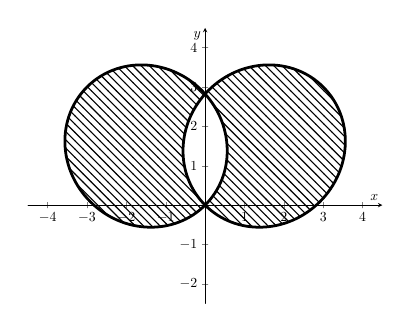
\begin{tikzpicture}[scale=0.5,line cap=round,line join=round,>=triangle 45,x=1cm,y=1cm]
\begin{axis}[
x=1cm,y=1cm,
axis lines=middle,
% ymajorgrids=true,
% xmajorgrids=true,
xmin=-4.5,
xmax=4.5,
ymin=-2.5,
ymax=4.5,
xtick={-5,-4,...,5},
ytick={-2,-1,...,4},]
\clip(-4.5,-2.5) rectangle (4.5,4.5);
% [color=ccqqqq]
\draw (1.4062674680691189,5.97677986476334) node[scale=3] {$f_2$} ;
\def\ellia{(-1.5,1.5) circle[x radius=2.121320343559643, y radius=2,rotate=-45]}
% \def\ellib{ (2,0) circle[x radius=2, y radius=1.7320508075688772,rotate=0]}
\def\ellib{(1.5,1.5) circle[x radius=2.121320343559643, y radius=2,rotate=45]}

\draw [line width=2pt] \ellia;
\draw [line width=2pt] \ellib;
\fill[pattern=north west lines ,even odd rule] \ellia \ellib;

\draw (4.3,0.2)  node[scale=1] {$x$};
\draw (-0.2,4.3)  node[scale=1] {$y$};

\end{axis}
\end{tikzpicture}
%     \caption{Graph of Example \ref{ex:twoellipses}}
%     \label{fig:twoellipses}
% \end{figure}
\vspace{-6mm}
\begin{figure}[h]
\begin{minipage}[htbp]{0.45\linewidth}
\begin{subfigure}
    \centering
    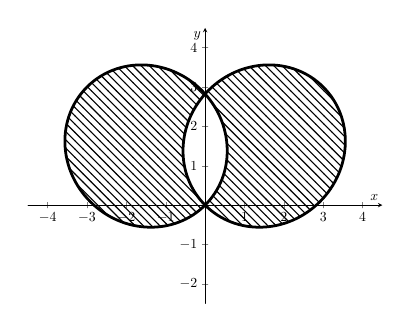
\begin{tikzpicture}[scale=0.5,line cap=round,line join=round,>=triangle 45,x=1cm,y=1cm]
\begin{axis}[
x=1cm,y=1cm,
axis lines=middle,
% ymajorgrids=true,
% xmajorgrids=true,
xmin=-4.5,
xmax=4.5,
ymin=-2.5,
ymax=4.5,
xtick={-5,-4,...,5},
ytick={-2,-1,...,4},]
\clip(-4.5,-2.5) rectangle (4.5,4.5);
% [color=ccqqqq]
\draw (1.4062674680691189,5.97677986476334) node[scale=3] {$f_2$} ;
\def\ellia{(-1.5,1.5) circle[x radius=2.121320343559643, y radius=2,rotate=-45]}
% \def\ellib{ (2,0) circle[x radius=2, y radius=1.7320508075688772,rotate=0]}
\def\ellib{(1.5,1.5) circle[x radius=2.121320343559643, y radius=2,rotate=45]}

\draw [line width=2pt] \ellia;
\draw [line width=2pt] \ellib;
\fill[pattern=north west lines ,even odd rule] \ellia \ellib;

\draw (4.3,0.2)  node[scale=1] {$x$};
\draw (-0.2,4.3)  node[scale=1] {$y$};

\end{axis}
\end{tikzpicture}
    \vspace{-5mm}
    \caption{The solution set of $F$ in Example \ref{ex:twoellipses}.
    %\ref{ex:twoellipses}
    }
    \label{fig:twoellipses}
\end{subfigure}
\end{minipage}
\hfill
\begin{minipage}[htbp]{0.45\linewidth}
\begin{subfigure}
    \centering
    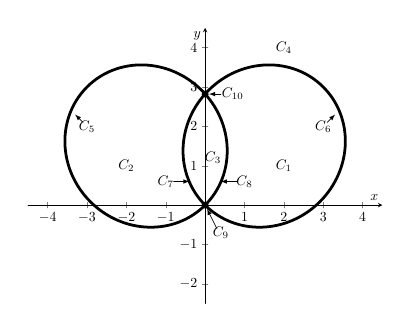
\begin{tikzpicture}[scale=0.5,line cap=round,line join=round,>=triangle 45,x=1cm,y=1cm]
\begin{axis}[
x=1cm,y=1cm,
axis lines=middle,
% ymajorgrids=true,
% xmajorgrids=true,
xmin=-4.5,
xmax=4.5,
ymin=-2.5,
ymax=4.5,
xtick={-5,-4,...,5},
ytick={-2,-1,...,4},]
\clip(-4.5,-2.5) rectangle (4.5,4.5);
% [color=ccqqqq]
\draw (1.4062674680691189,5.97677986476334) node[scale=3] {$f_2$} ;
\def\ellia{(-1.5,1.5) circle[x radius=2.121320343559643, y radius=2,rotate=-45]}
% \def\ellib{ (2,0) circle[x radius=2, y radius=1.7320508075688772,rotate=0]}
\def\ellib{(1.5,1.5) circle[x radius=2.121320343559643, y radius=2,rotate=45]}
\fill (0,0) circle (2.5pt);
\fill (0,2.82) circle (2.5pt);
\draw (2,1)  node[scale=1] {$C_1$};
\draw (-2,1)  node[scale=1] {$C_2$};
\draw (0.2,1.2)  node[scale=1] {$C_3$};

\draw (2,4)  node[scale=1] {$C_4$};
\draw (-3,2) node[scale=1] {$C_5$};
\draw [-latex,line width=0.5pt]  (-3.1,2.1) -- (-3.3,2.3);
\draw (3,2) node[scale=1] {$C_6$};
\draw [-latex,line width=0.5pt]  (3.1,2.1) -- (3.3,2.3);
\draw (-1, 0.6) node[scale=1] {$C_7$};
\draw [-latex,line width=0.5pt]  (-0.8,0.6) -- (-0.4,0.6);
\draw (1, 0.6) node[scale=1] {$C_8$};
\draw [-latex,line width=0.5pt]  (0.8,0.6) -- (0.4,0.6);
\draw (0.4,-0.7) node[scale=1] {$C_9$};
\draw [-latex,line width=0.5pt]  (0.3,-0.6) -- (0.05,-0.1);
\draw (0.7,2.82) node[scale=1] {$C_{10}$};
\draw [-latex,line width=0.5pt]  (0.4,2.82) -- (0.1,2.82);

\draw [line width=2pt] \ellia;
\draw [line width=2pt] \ellib;
% \fill[pattern=north west lines ,even odd rule] \ellia \ellib;

\draw (4.3,0.2)  node[scale=1] {$x$};
\draw (-0.2,4.3)  node[scale=1] {$y$};

\end{axis}
\end{tikzpicture}
    \vspace{-5mm}
    \caption{The zero level set of $\poly(F)$ decomposes $\R^2$ into $10$ cells.}
    \label{fig:twoellipses2}
\end{subfigure}
\end{minipage}

\end{figure}
\end{example}
\vspace{-11mm}

\begin{definition}[Cell]\label{def:cell}
% Let $Q\subseteq\R[\vX]$ and $\bar{a}\in \R^n$ a \textcolor{blue}{sample point}.
% Consider a set of  polynomials $Q\subseteq\R[\vX]$ and a sample $\bar{a}\in \R^n$. 
For any finite set $Q\subseteq\R[\vX]$, a \emph{cell} of $Q$ is
a maximally connected set in $\R^{n}$ on which the sign of every polynomial in $Q$ is constant.
%is called a cell of $Q$.  
% \textcolor{blue}{
% Any point in a cell is called a \emph{sample point} of the cell.}
For any point $\bar{a}\in\R^{n}$,
we denote by $\cell{Q}{\bar{a}}$ the cell of $Q$ containing $\bar{a}$. 
\end{definition}
\vspace{-2mm}

By the theory of CAD, we have 
\vspace{-2mm}
\begin{corollary}
For any finite set $Q\subseteq \R[\vX]$, the number of cells of $Q$ is finite.
\end{corollary}
\vspace{-2mm}
%\begin{proof} 
%According to the theory of CAD, the cells of $Q$ are finitely many.
%\end{proof}

It is obvious that any two cells of $Q$ are disjoint and the union of all cells of $Q$ equals $\R^{n}$.
Definition \ref{def:cell} shows that
for a polynomial formula $F$ with $\poly(F)=Q$,
the satisfiability of $F$ is constant on every cell of $Q$, that is, either all the points in a cell are  solutions to $F$ or none of them are solutions to $F$.

% the points in a cell are either solutions to $F$ or not solutions to $F$. 
% Suppose $F$ is a polynomial formula such that $\poly(F)=Q$.
% \textcolor{blue}{===============}
% Easy to known, the cells of $Q$ are disjoint and cover R. It can be seen that for any formula f composed of Q, in any cell c of Q, feasibility is consistent, meaning either all points in c are feasible or all points in c are infeasible.
% \textcolor{red}{===============}
\vspace{-2mm}

\begin{example}\label{ex:twoellipses2} 
% $$f=17x^2 + 2xy + 17y^2 + 48x - 48y;\ g=3x^2 + 4y^2 - 12x;$$

Consider the polynomial formula $F$
%Continuing with the formula $\varphi$  
in Example \ref{ex:twoellipses}. 
As shown in Figure \ref{fig:twoellipses3}, assume that we start from point $a$ to search for a solution to $F$.
Jumping from $a$ to $b$ makes no difference, as both points are in the same cell and thus neither are solutions to $F$.
% if we want to search for its solution on $R^2$ starting from point a (as shown in Figure \ref{fig:twoellipses3}), then the jump from a to b has no meaning, as they are in the same cell and will not change the feasibility state. 
However, jumping from $a$ to $c$ or from $a$ to $d$ %is different, since it 
crosses different cells and we may discover a cell satisfying $F$.
% as they cross cells, and it is possible to discover different states, where 
Herein, the cell containing $d$ satisfies $F$.
% \vspace{-6mm}
\begin{figure}[h]
    \begin{minipage}[htbp]{0.45\linewidth}
        \begin{subfigure}
            \centering
            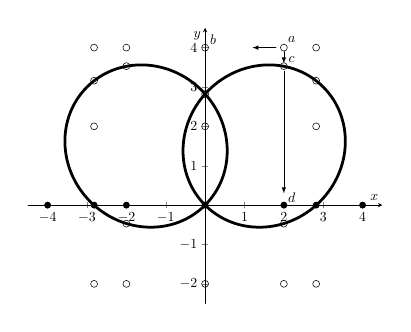
\begin{tikzpicture}[scale=0.5,line cap=round,line join=round,>=triangle 45,x=1cm,y=1cm]
\begin{axis}[
x=1cm,y=1cm,
axis lines=middle,
% ymajorgrids=true,
% xmajorgrids=true,
xmin=-4.5,
xmax=4.5,
ymin=-2.5,
ymax=4.5,
xtick={-5,-4,...,5},
ytick={-2,-1,...,4},]
\clip(-4.5,-2.5) rectangle (4.5,4.5);
% [color=ccqqqq]
\draw (1.4062674680691189,5.97677986476334) node[scale=3] {$f_2$} ;
\def\ellia{(-1.5,1.5) circle[x radius=2.121320343559643, y radius=2,rotate=-45]}
% \def\ellib{ (2,0) circle[x radius=2, y radius=1.7320508075688772,rotate=0]}
\def\ellib{(1.5,1.5) circle[x radius=2.121320343559643, y radius=2,rotate=45]}

\draw [line width=2pt] \ellia;
\draw [line width=2pt] \ellib;
% \fill[pattern=north west lines ,even odd rule] \ellia \ellib;

\draw (2,4)   circle (2.5pt);
\draw (2.2,4.2)  node[scale=1] {$a$};
\draw (0,4)   circle (2.5pt);
\draw (0.2,4.2)  node[scale=1] {$b$};
\draw [-latex,line width=0.5pt]  (1.8,4) -- (1.2,4);
\draw (2,3.53)   circle (2.5pt);
\draw (2.2,3.7)  node[scale=1] {$c$};
\draw [-latex,line width=0.5pt]  (2,3.9) -- (2,3.6);
% \draw (2,2)   circle (2.5pt);
\draw (2.2,0.2)  node[scale=1] {$d$};

\draw [-latex,line width=0.5pt]  (2,3.4) -- (2,0.3);
\fill (0,0) circle (2.5pt);
\draw (0,-2)   circle (2.5pt);
\draw (0,2)   circle (2.5pt);
\draw (0,2.82)   circle (2.5pt);
% \draw (0,4)   circle (2.5pt);

\fill (2,0) circle (2.5pt);
\draw (2,-0.47)   circle (2.5pt);
\draw (2,-2)   circle (2.5pt);

\fill (2.82,0) circle (2.5pt);
\draw (2.82,-2)   circle (2.5pt);
\draw (2.82,2)   circle (2.5pt);
\draw (2.82,3.16)   circle (2.5pt);
\draw (2.82,4)   circle (2.5pt);

\fill (4,0) circle (2.5pt);
\fill (-2,0) circle (2.5pt);
\draw (-2,-0.47)   circle (2.5pt);
\draw (-2,-2)   circle (2.5pt);
\draw (-2,4)   circle (2.5pt);
\draw (-2,3.53)   circle (2.5pt);

\fill (-2.82,0) circle (2.5pt);
\draw (-2.82,-2)   circle (2.5pt);
\draw (-2.82,2)   circle (2.5pt);
\draw (-2.82,3.16)   circle (2.5pt);
\draw (-2.82,4)   circle (2.5pt);

\fill (-4,0) circle (2.5pt);

\draw (4.3,0.2)  node[scale=1] {$x$};
\draw (-0.2,4.3)  node[scale=1] {$y$};


\end{axis}
\end{tikzpicture}
            \vspace{-5mm}
            \caption{Jumping from point $a$ to search for a solution of $F$.
            }
            \label{fig:twoellipses3}
        \end{subfigure}
    \end{minipage}
    \hfill
    \begin{minipage}[htbp]{0.45\linewidth}
        \begin{subfigure}
            \centering
            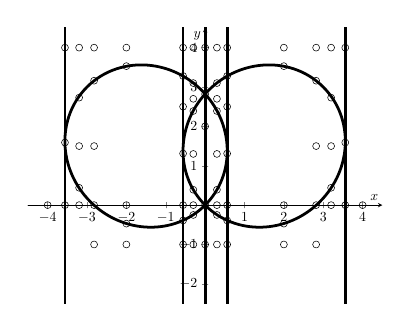
\begin{tikzpicture}[scale=0.5,line cap=round,line join=round,>=triangle 45,x=1cm,y=1cm]
\begin{axis}[
x=1cm,y=1cm,
axis lines=middle,
% ymajorgrids=true,
% xmajorgrids=true,
xmin=-4.5,
xmax=4.5,
ymin=-2.5,
ymax=4.5,
xtick={-5,-4,...,5},
ytick={-2,-1,...,4},]
\clip(-4.5,-2.5) rectangle (4.5,4.5);
% [color=ccqqqq]
\draw (1.4062674680691189,5.97677986476334) node[scale=3] {$f_2$} ;
\def\ellia{(-1.5,1.5) circle[x radius=2.121320343559643, y radius=2,rotate=-45]}
% \def\ellib{ (2,0) circle[x radius=2, y radius=1.7320508075688772,rotate=0]}
\def\ellib{(1.5,1.5) circle[x radius=2.121320343559643, y radius=2,rotate=45]}

\draw [line width=2pt] \ellia;
\draw [line width=2pt] \ellib;
% \fill[pattern=north west lines ,even odd rule] \ellia \ellib;

% -3.56155}, {x -> -0.561553}, {x -> 0}, {x -> 0.561553}, {x -> 
%    3.56155}}
   
\draw [line width=2pt]  (-3.56,-3) -- (-3.56,6);
\draw [line width=2pt]  (-0.56,-3) -- (-0.56,6);
\draw [line width=2pt]  (0,-3) -- (0,6);
\draw [line width=2pt]  (0.56,-3) -- (0.56,6);
\draw [line width=2pt]  (3.56,-3) -- (3.56,6);


\draw (4.3,0.2)  node[scale=1] {$x$};
\draw (-0.2,4.3)  node[scale=1] {$y$};


\draw (2,4)   circle (2.5pt);
\draw (0,4)   circle (2.5pt);
\draw (2,3.53)   circle (2.5pt);

\draw (0,0) circle (2.5pt);
\draw (0,-1)   circle (2.5pt);
\draw (0,2)   circle (2.5pt);
\draw (0,2.82)   circle (2.5pt);
% \draw (0,4)   circle (2.5pt);

\draw (2,0) circle (2.5pt);
\draw (2,-0.47)   circle (2.5pt);
\draw (2,-1)   circle (2.5pt);

\draw (2.82,0) circle (2.5pt);
\draw (2.82,-1)   circle (2.5pt);
\draw (2.82,1.5)   circle (2.5pt);
\draw (2.82,3.16)   circle (2.5pt);
\draw (2.82,4)   circle (2.5pt);

\draw (4,0) circle (2.5pt);
\draw (-4,0) circle (2.5pt);

\draw (-2,0) circle (2.5pt);
\draw (-2,-0.47)   circle (2.5pt);
\draw (-2,-1)   circle (2.5pt);
\draw (-2,4)   circle (2.5pt);
\draw (-2,3.53)   circle (2.5pt);

\draw (-2.82,0) circle (2.5pt);
\draw (-2.82,-1)   circle (2.5pt);
\draw (-2.82,1.5)   circle (2.5pt);
\draw (-2.82,3.16)   circle (2.5pt);
\draw (-2.82,4)   circle (2.5pt);

\draw (-0.56,-1)   circle (2.5pt);
\draw (-0.56,-0.39)   circle (2.5pt);
\draw (-0.56,0) circle (2.5pt);
\draw (-0.56,1.31)   circle (2.5pt);
\draw (-0.56,2.5)   circle (2.5pt);
\draw (-0.56,3.28)   circle (2.5pt);
\draw (-0.56,4)   circle (2.5pt);

\draw (0.56,-1)   circle (2.5pt);
\draw (0.56,-0.39)   circle (2.5pt);
\draw (0.56,0) circle (2.5pt);
\draw (0.56,1.31)   circle (2.5pt);
\draw (0.56,2.5)   circle (2.5pt);
\draw (0.56,3.28)   circle (2.5pt);
\draw (0.56,4)   circle (2.5pt);

\draw (-3.56,0)   circle (2.5pt);
% \draw (-3.56,0.7)   circle (2.5pt);
\draw (-3.56,1.59)   circle (2.5pt);
\draw (-3.56,4)   circle (2.5pt);
\draw (3.56,0)   circle (2.5pt);
% \draw (3.56,0.7)   circle (2.5pt);
\draw (3.56,1.59)   circle (2.5pt);
\draw (3.56,4)   circle (2.5pt);

\draw (-3.2,0)   circle (2.5pt);
\draw (-3.2,0.44)   circle (2.5pt);
\draw (-3.2,1.5)   circle (2.5pt);
\draw (-3.2,2.73)   circle (2.5pt);
\draw (-3.2,4)   circle (2.5pt);
\draw (3.2,0)   circle (2.5pt);
\draw (3.2,0.44)   circle (2.5pt);
\draw (3.2,1.5)   circle (2.5pt);
\draw (3.2,2.73)   circle (2.5pt);
\draw (3.2,4)   circle (2.5pt);


\draw (-0.3,-1)   circle (2.5pt);
\draw (-0.3,-0.25)   circle (2.5pt);
\draw (-0.3,0)   circle (2.5pt);
\draw (-0.3,0.39)   circle (2.5pt);
\draw (-0.3,1.3)   circle (2.5pt);
\draw (-0.3,2.39)   circle (2.5pt);
\draw (-0.3,2.7)   circle (2.5pt);
\draw (-0.3,3.1)   circle (2.5pt);
\draw (-0.3,4)   circle (2.5pt);
\draw (0.3,-1)   circle (2.5pt);
\draw (0.3,-0.25)   circle (2.5pt);
\draw (0.3,0)   circle (2.5pt);
\draw (0.3,0.39)   circle (2.5pt);
\draw (0.3,1.3)   circle (2.5pt);
\draw (0.3,2.39)   circle (2.5pt);
\draw (0.3,2.7)   circle (2.5pt);
\draw (0.3,3.1)   circle (2.5pt);
\draw (0.3,4)   circle (2.5pt);

\end{axis}
\end{tikzpicture}
            \vspace{-5mm}
            \caption{A cylindrical expansion of a cylindrically complete set containing $\poly(F)$.}
            \label{fig:twoellipses4}
        \end{subfigure}
    \end{minipage}
\end{figure}
% \vspace{-10mm}
\end{example}
%\vspace{-3mm}

%Cells in SMT(NRA) are similar to Boolean assignments in SAT,  since both are finitely many and crucial for determining the satisfiability of the formula. We view these cells as \emph{states} for NRA.  By analogy with a search procedure for SAT that jumps between different Boolean assignments, one for SMT(NRA) should jump between different cells.


% By analogy with a search procedure for SAT that jumps between different Boolean assignments, one for SMT(NRA) should jump between different cells.
% % The key point is to define an operation to travel these cells. 
% % We will propose such an jumping operation, called \emph{cell-jump}, 
% %for jumping between different cells 
% % in the next section. 
% %along with some related heuristic strategies.
% In the rest of this section, we will %demonstrate 
% give a search strategy through point jumping to traverse all cells.
% The strategy will be explained step by step in Def. \ref{def:expansion}--Def. \ref{def:cyl_complete}.
% This is indeed a thing with very high cost, in the worst case, it will have an exponential complexity.
% how to traverse all cells through point jumping. 
% That is, just as there exists a complete strategy for traversing the entire boolean space through flipping of boolean values in SAT, there also exists a basic strategy for traversing all cells through point jumps between cells. Certainly, for efficiency considerations, we would adopt a heuristic approach to jumping.
% For any $Q\subseteq\R[\vX]$ and any point $\vA=(a_1,\ldots,a_n)\in\R^n$,    
% $\sub{Q}{\vA}{x_i}$ denotes 
% the set $\{q(a_1,\ldots,a_{i-1},x_i,a_{i+1},\ldots,a_n)\mid q\in Q\}$.
% and $\vA_{(i)}$ denotes the $i$-component $a_i$ of $\vA$.
% $Q[x_1/a_1,\ldots,x_{i-1}/a_{i-1},x_{i+1}/a_{i+1},\ldots,x_n/a_n]$.



% \textcolor{red}{We will introduce this operation for jumping between different cells in the next section, along with some related heuristic strategies.}

For the remainder of this section, we will demonstrate how to traverse all cells through point jumps between cells. %That is, just as there exists a complete strategy for traversing the entire Boolean space through flipping of Boolean values in SAT, there also exists a basic strategy for traversing all cells through point jumps between cells. %Certainly, for efficiency considerations, we would adopt a heuristic approach to jumping.
The method essentially traversing cell by cell in a variable by variable direction will be explained step by step from Definition \ref{def:expansion} to Definition \ref{def:cyl_complete}. %In the worst case, it will have an exponential complexity. %First, we describe the set of points that a point may generate by jump from cell to cell on one variable direction.
%\vspace{-2mm}
\begin{definition}[Expansion]\label{def:expansion}
Let $Q\subseteq\R[\vX]$ be finite and $\bar{a}=(a_1,\ldots,a_n)\in \R^n$. 
Given a variable $x_i~(1\le i\le n)$, let $r_1<\cdots<r_s$ be all real roots of $\{q(a_1,\ldots,a_{i-1},x_i,\allowbreak a_{i+1},\ldots,a_n)\mid q(a_1,\ldots,a_{i-1},x_i,\allowbreak a_{i+1},\ldots,a_n)\not\equiv 0,\  q\in Q\}$,
%$\sub{Q}{\vA}{x_i}$, 
where $s\in\Z_{\ge0}$. 
An \emph{expansion} of $\bar{a}$ to $x_i$ on $Q$ is a point set $\Lambda\subseteq \R^n$ satisfying 

\vspace{-2mm}
\begin{enumerate}[label=$($\alph*$)$]
    \item $\bar{a}\in \Lambda$ and  $(a_1,\ldots,a_{i-1},r_j,a_{i+1},\ldots,a_n)\in \Lambda$ for $1\leq j\leq s$,
    \item for any $\bar{b}=(b_1,...,b_n)\in \Lambda$,
    $b_j=a_j$ for $j\in\{1,\ldots,n\}\setminus\{i\}$, and
    \item
    for any interval  $I\in\{(-\infty,r_1),(r_1,r_2),\ldots,(r_{s-1},r_s),(r_s,+\infty)\}$,
    there exists unique $\bar{b}=(b_1,...,b_n)\in \Lambda$ such that $b_i\in I.$ 
    % $r_{j}<b_i<r_{j+1}$ for  $1\leq j < s$, $b_i<r_1$ and  $b_i>r_s$,
    % \item there exists unique $\bar{b}\in \Lambda$ such that $b_i<r_1$, and
    % \item there exists unique $\bar{b}\in \Lambda$ such that $b_i>r_s$,
\end{enumerate}
\vspace{-2mm}
% where $b_i$ is the $i$-th component of $\bar{b}$.
For any point set $\{\vA^{(1)},\ldots,\vA^{(m)}\}\subseteq\R^{n}$, an \emph{expansion} of the set to $x_i$ on $Q$ is $\bigcup_{j=1}^m\Lambda_j$, where $\Lambda_j$ is an expansion of $\vA^{(j)}$ to $x_i$ on $Q$.
\end{definition} 
\vspace{-3mm}
\begin{example}\label{ex:expansion} 
Consider the polynomial formula $F$
in Example \ref{ex:twoellipses}.  
The set of black solid points in Figure \ref{fig:twoellipses3}, denoted as $\Lambda$, is an expansion of point $(0,0)$ to $x$ on $\poly(F)$.
The set of all points (including black solid points and hollow points) is an expansion of $\Lambda$ to $y$ on $\poly(F)$.
\end{example}
\vspace{-2mm}

As shown in Figure \ref{fig:twoellipses3},  an expansion of a point   to some variable  is actually a result of the point continuously jumping to adjacent cells along that variable direction.
Next, we describe the expansion of all variables in order, which is a result of jumping from cell to cell along the directions of variables w.r.t. a variable order.
% For any polynomial formula $F$,
% given a starting point $\vA\in\R^{n}$ and some variable $x_i$, 
% the first step of the search strategy jumps to every point in an expansion of $\vA$ to $x_i$ on $\poly(F)$.
% As shown in Figure \ref{fig:twoellipses3}, 
% \textcolor{red}{
% an expansion of a point $(a_1,\ldots,a_n)$ in $\R^{n}$ to some variable $x_i$ 
% represents all the cells that intersects 
% the line $(a_1,\ldots,a_{i-1},\R,a_{i+1},\ldots,a_n)$.}
% Thus, every point in the expansion is a candidate point for jumping.
% consists of candidate points for jumping 
%is actually a kind of jump from the point to
% \textcolor{red}{all accessible cavities} in 
\vspace{-2mm}
\begin{definition}[Cylindrical Expansion]\label{def:cyl_expansion}
Let $Q\subseteq\R[\vX]$ be finite and $\bar{a}\in \R^n$. 
Given a variable order $x_1\prec\cdots\prec x_n$, 
a \emph{cylindrical expansion} of $\bar{a}$ w.r.t. the variable order on $Q$
is $\bigcup_{i=1}^n \Lambda_i$, where 
$\Lambda_1$ is an expansion of $\bar{a}$ to $x_1$ on $Q$, and
for $1\leq i<n$, $\Lambda_{i+1}$ is an expansion of $\Lambda_{i}$ to $x_{i+1}$ on $Q$.
% \begin{enumerate}[label=$($\alph*$)$]
%     \item $\Lambda_1$ is an expansion of $\bar{a}$ to $x_1$ on $Q$, and
%     \item for $1\leq i<n$, $\Lambda_{i+1}$ is an expansion of $\Lambda_{i}$ to $x_{i+1}$ on $Q$.
% \end{enumerate}
% We also call  a \emph{cylindrical sample set} of $Q$.
When the context is clear, we simply call
% Under no ambiguity, we refer to
$\bigcup_{i=1}^n \Lambda_i$ a \emph{cylindrical expansion} of $Q$.
\end{definition}
\vspace{-3mm}
\begin{example}\label{ex:cyl_expansion} 
Consider the formula $F$
in Example \ref{ex:twoellipses}.  
%Recalling Example \ref{ex:expansion}, 
It is clear that the set of all points 
%(including black solid points and hollow points) 
in Figure \ref{fig:twoellipses3} is a cylindrical expansion of point $(0,0)$ w.r.t. $x\prec y$ on $\poly(F)$.
% , where $F$ is the polynomial formula in Example \ref{ex:twoellipses}.
%for any polynomial formula $F$, 
The expansion actually describes the following jumping process. First, the origin $(0,0)$ jumps along the $x$-axis to the black points, and then those black points jump along the $y$-axis direction to the white points.
%Note that the points in the cylindrical expansion cover all the cells except $C_7$ and $C_8$ (see Figure \ref{fig:twoellipses2}). 
% then the cells 
% $C_7$ and $C_8$ cannot be traversed (see Figure \ref{fig:twoellipses2}).
% Thus, we need the following definition and Theorem \ref{thm:CAD} to guarantee to cover all cells. 
\end{example}
\vspace{-2mm}

Clearly, a cylindrical expansion is %a result of a point jumping recursively from one variable to another. 
similar to how a Boolean vector is flipped variable by variable. Note that the points in the expansion in Figure \ref{fig:twoellipses3} do not cover all the cells ({\it e.g.} $C_7$ and $C_8$ in Figure \ref{fig:twoellipses2}), but if we start from $(0,2)$, all the cells can be covered. This implies that whether all the cells can be covered depends on the starting point. %, because some polynomial sets lack some projections.

% \begin{corollary}
% Let $Q\subseteq\R[\vX]$.
% For any cylindrical sample set $\Lambda$ of $Q$, the cells containing a point of $\Lambda$ are pairwise disjoint.
% \end{corollary}
\vspace{-2mm}
\begin{definition}[Cylindrically Complete]\label{def:cyl_complete}
Let $Q\subseteq\R[\vX]$ be finite.
Given a variable order $x_1\prec\cdots\prec x_n$, 
$Q$ is said to be \emph{cylindrically complete} w.r.t. the variable order,
if for any $\vA\in \R^n$ and for any cylindrical expansion $\Lambda$ of $\vA$ w.r.t. the order on $Q$,
every cell of $Q$ contains at least one point in $\Lambda$. 
\end{definition}
\vspace{-4mm}
\begin{theorem}\label{thm:CAD}
For any finite set $Q\subseteq\R[\vX]$ and any variable order, 
there exists %a set 
$Q'$ such that $Q\subseteq Q'\subseteq\R[\vX]$ and $Q'$ is cylindrically complete w.r.t. the variable order.
\end{theorem}
\vspace{-4mm}

\begin{proof} 
Let $Q'$ be the projection set of $Q$ \cite{collins1975quantifier,mccallum1998improved,brown2001improved} obtained from the CAD projection operator w.r.t. the variable order.
%is denoted as $Q'$. 
According to the theory of CAD, $Q'$ is cylindrically complete.\hfill$\square$
\end{proof}
\vspace{-4mm}

\begin{corollary}\label{coro:CAD}
For any polynomial formula $F$ and any variable order,
% and any variable order, 
there exists a finite set $Q\subseteq\R[\vX]$ such that  for any cylindrical expansion $\Lambda$ of $Q$, every cell of $\poly(F)$ contains at least one point in $\Lambda$. 
Furthermore, $F$ is satisfiable if and only if 
$F$ has solutions in  $\Lambda$.
\end{corollary}
\vspace{-4mm}
%  

\begin{example} 
Consider the polynomial formula $F$
in Example \ref{ex:twoellipses}.
By the proof of Theorem \ref{thm:CAD}, $Q':=\{
x, -2 - 3 x + x^2,\; -2 + 3 x + x^2,\; 
 10944 + 17 x^2,\; %-48 x + 17 x^2 - 48 y - 2 x y + 17 y^2, \;
 %48 x + 17 x^2 - 48 y + 2 x y + 17 y^2
f_1,\; f_2\}$ is a cylindrically complete set w.r.t. $x\prec y$
containing $\poly(F)$.
As shown in Figure \ref{fig:twoellipses4}, the set of all (hollow) points is a cylindrical expansion of point $(0,0)$ w.r.t. $x \prec y$ on $Q'$, which 
% covers all cells of $Q'$, and thus 
covers all cells of $\poly(F)$.
\end{example}
\vspace{-2mm}


Corollary \ref{coro:CAD} shows that for a polynomial formula $F$, there exists a finite set $Q\subseteq\R[\vX]$ such that we can traverse all the cells of $\poly(F)$ through a search path containing all points in a cylindrical expansion of $Q$.  The cost of traversing the cells is very high, and in the worst case, the number of cells will grow exponentially with the number of variables.

The key to building a local search on SMT(NRA) is to construct a heuristic search based on the operation of jumping between cells. %We will introduce in the following sections a jump operation between cells, called \emph{cell-jump}, and the heuristic search built based on it.

% However, it is inefficient to compute $Q$ in practice.
% So, we use a search strategy jumping between the points in a cylindrical expansion of $\poly(F)$, although the strategy may omit some cells (see Example \ref{ex:cyl_expansion}).

% define an operation, called \emph{cell-jump}, for jumping between different cells 
% in the next section without computing $Q$. 
%along with some related heuristic strategies.

\begin{comment}
Applying a local search procedure to solve SMT(NRA), the search space is $\R^{n}$ which consists of infinite candidate assignments.
However, the method of cylindrical algebraic decomposition, CAD for short, guarantees the search space only has finite states in theory.

For any finite set of polynomials in $\Q[\vX]$,
there exists a cylindrical algebraic decomposition w.r.t. it,
which is a decomposition of $\R^n$ into finite cells such that each polynomial has constant sign on each cell.
% And thus, the $i$-th cell has a constant sign sequence $[s_{i1},\ldots,s_{im}]$, where $s_{ij}$ is the sign of $p_j$ on it.
Take the set with a single polynomial $h=2x_{1}^4 + x_{2}^4 - 3x_{1}^2x_{2} - 2x_{2}^3 + x_{2}^2$ for example.
Figure \ref{fig:CAD} $($a$)$ shows the graph of $h=0$ (curve $e$ in the figure) decomposes $\R^2$ into $5$ cells: area $a$, area $b$, area $c$, area $d$ and curve $e$. 
The signs of $h$ on them are $+$, $-$, $-$, $+$ and $0$, respectively.  
So, the $5$ cells form a cylindrical algebraic decomposition %of $\R^{2}$ w.r.t. $\{h\}$.
% , those have sign sequences $[+]$, $[-]$, $[-]$, $[+]$ and $[0$, respectively. 

\begin{figure}[ht]
\centering
\subfigure[]
    {
        \centering
        \includegraphics[scale=0.8]{fig/CAD_cells.pdf}
    }
\subfigure[]
    {
    \centering
    \includegraphics[scale=0.8]{fig/CAD_states.pdf}
    }
\caption{The graph of $h=0$, where $h=2x_{1}^4 + x_{2}^4 - 3x_{1}^2x_{2} - 2x_{2}^3 + x_{2}^2$.
%decomposes $\R^2$ into $5$ cells.
(The horizontal axis denotes the $x_1$-axis and the vertical one denotes the $x_2$-axis.)
}
\label{fig:CAD}
\end{figure}

% \begin{figure}[ht]
% \centering
% \includegraphics[width=4.5cm]{fig/CAD.pdf}
% \caption{The graph of $2x_{1}^4 + x_{2}^4 - 3x_{1}^2x_{2} - 2x_{2}^3 + x_{2}^2=0$ decomposes $\R^2$ into $5$ cells.
% (The horizontal axis denotes the $x_1$-axis and the vertical one denotes the $x_2$-axis.)
% }
% \label{fig:CAD}
% \end{figure}

We now define \emph{states} of the search space $\R^{n}$. 
%w.r.t. a polynomial formula.
For any polynomial formula $F$ with polynomials $\{p_1,\ldots,p_m\}$,
every cell in a CAD w.r.t. $\{p_1,\ldots,p_m\}$ gives a sign sequence $[s_{i1},\ldots,s_{im}]$, where $i$ denotes the serial number of the cell and $s_{ij}$ is the constant sign of $p_{j}$ on the cell.
If there is a sign sequence satisfying $F$,
then any point from the cells with the sign sequence is a solution to $F$.
Therefore, we define \emph{states} of the search space $\R^{n}$ as unions of cells with the same sign sequence, the number of those is finite since that of cells is.
Take the formula $h>0$ for instance.
Although there are $5$ cells in the CAD w.r.t. $\{h\}$,
it only has $3$ states: 
the union of area $a$ and area $d$,
the union of area $b$ and area $c$, and
curve $e$ (also see state \uppercase\expandafter{\romannumeral1}, state \uppercase\expandafter{\romannumeral2} and state \uppercase\expandafter{\romannumeral3} in Figure \ref{fig:CAD} $($b$)$, respectively).
Only points in state \uppercase\expandafter{\romannumeral1} are solutions to $h>0$.

From the perspective of CAD, the search space of SMT(NRA) consists of finite states.
We emphasize that we do not compute cylindrical algebraic decomposition in our proposed local search algorithm, because of its doubly-exponential complexity. 
CAD just gives a new view to local search on $\R^{n}$: Moving from assignment to assignment in $\R^n$ is essentially moving between finitely many states.
\end{comment}
% From the perspective of CAD,
% to find a solution of a given polynomial formula $F$ is essentially to find a cell with a satisfied sign sequence. 
% %of signs of all polynomials appearing in it.
% More concretely,
% we denote all polynomials appearing in the formula $p_1,\ldots,p_m$.
% %and
% % Given a polynomial formula $F$,
% % we put all polynomials appearing in it in a set $\{p_1,\ldots,p_m\}$.
% A cylindrical algebraic decomposition w.r.t $\{p_1,\ldots,p_m\}$
% % which decomposes $\R^{n}$ into $r$ cells, 
% gives a set of candidate sign sequences $S=\{[s_{i1},\ldots,s_{im}]\mid s_{ij}~{\rm is~the~sign~of}~p_j~{\rm on~the}~i-{\rm th~cell}\}$.
% % Every sign sequence in $S$ corresponds to a state, that is the union of cells.
% Any element from $S$ that satisfies the given formula is a satisfied sign sequence, and if there exists no such one in $S$, CAD ensures that the formula is unsatisfied over the reals.
% , the number of those are is equal to the cardinality of $S$.
% Take the formula $h>0$ for instance.
% The CAD of $\{h\}$ gives candidate sign sequences $[+],[]$
\vspace{-4mm}
\section{The Cell-Jump Operation}\label{sec:cell_jump}
\vspace{-2mm}

% Inspired by the %literal-level
% \emph{critical move} operation \cite[Definition 2]{cai2022local} which is proposed in a local search algorithm for solving satisfiability of LIA formulas, 
In this section, we propose a novel operation, called \emph{cell-jump}, 
that performs local changes in our algorithm.
% for polynomial formulas.
% Both operators modify the value of a variable by a fixed increment.
% Since the case of polynomial formulas is complicated, 
The operation is determined by the means of real root isolation.
We review the method of real root isolation and define \emph{sample points} in Section \ref{subsec:realrootiso}.
Section \ref{subsec:celljump} and Section \ref{subsec:cell_jump_dir} present a cell-jump operation along a line parallel to a coordinate axis and along any fixed straight line, respectively.
% Then, we define a cell-jump operation along a line parallel to a coordinate axis and along any fixed straight line in Section \ref{subsec:celljump} and Section \ref{subsec:cell_jump_dir}, respectively.
\vspace{-5mm}
\subsection{Sample Points}\label{subsec:realrootiso}
\vspace{-2mm}
Real root isolation is a symbolic way to compute the real roots of a polynomial, which is of fundamental importance in computational real algebraic geometry ({\it e.g.}, it is a routing sub-algorithm for CAD).
There are many efficient algorithms and popular tools in computer algebra systems such as  Maple and Mathematica to isolate the real roots of polynomials.
% In this paper, we only consider real root isolation of univariate polynomials. %and 

We first introduce the definition of \emph{sequences of isolating intervals} for nonzero univariate polynomials,
which can be obtained by any real root isolation tool. %, {\it e.g.} CLPoly.
%\footnote{\url{https://github.com/lihaokun/CLPoly}.}.
% In fact, for any nonzero univariate polynomial $p(x)\in\Q[x]$, we can obtain a sequence of isolating intervals of $p(x)$ by a real root isolation algorithm.
% \textcolor{blue}{
% Formally, given , a real root isolation algorithm computes a \emph{sequence of isolating intervals} of $p(x)$. }
% \vspace{-2mm}
\begin{definition}[\bf Sequence of Isolating Intervals]
For any nonzero univariate polynomial $p(x)\in\Q[x]$, a \emph{sequence of isolating intervals} of $p(x)$ is a sequence of open intervals $(a_1,b_1),\ldots,(a_s,b_s)$ where $s\in\Z_{\ge0}$, such that
\vspace{-1.5mm}
\begin{enumerate}
    \item for each $i~(1\le i\le s)$, $a_i,b_i\in\Q$, $a_i< b_i$ and $b_i < a_{i+1}$, 
    \item each interval $(a_i,b_i)~(1\le i\le s)$ has exactly one real root of $p(x)$, and
    \item none of the real roots of $p(x)$ are in $\R\setminus\bigcup_{i=1}^{s}(a_i,b_i)$.
\end{enumerate}
\vspace{-1.5mm}
Specially, the sequence of isolating intervals is empty, {\it i.e.}, $s=0$, when $p(x)$ has no real roots.
\end{definition}
\vspace{-2mm}

By means of sequences of isolating intervals, we define \emph{sample points} of univariate polynomials, which is the key concept of the \emph{cell-jump} operation proposed in Section \ref{subsec:celljump} and Section \ref{subsec:cell_jump_dir}. 
% \vspace{-2mm}
\begin{definition}[\bf Sample Point]\label{def:sample_points}
For any nonzero univariate polynomial $p(x)\in\Q[x]$, let $(a_1,b_1),\ldots,(a_s,b_s)$ be a sequence of isolating intervals of $p(x)$ where $s\in\Z_{\ge0}$.
Every point in the set $\{a_1,b_s\}\cup\bigcup_{i=1}^{s-1}\{b_i,\frac{b_i+a_{i+1}}{2},a_{i+1}\}$ is a \emph{sample point} of $p(x)$.
If $x^{*}$ is a sample point of $p(x)$ and $p(x^{*})>0$ $($or $p(x^{*})<0)$, then $x^{*}$ is a \emph{positive sample point} $($or \emph{negative sample point}$)$ of $p(x)$. 
For the zero polynomial, it has no \emph{sample point}, no \emph{positive sample point} and no \emph{negative sample point}.
\end{definition}
\vspace{-4mm}
\begin{remark}\label{remark:about_sample_points}
% Let the notation be the same as in Definition \ref{def:sample_points}.
For any nonzero univariate polynomial $p(x)$ that has real roots,
% if it , then it has no sample points.
% Otherwise, 
let $r_1,\ldots,\allowbreak r_s\;(s\in\Z_{\ge1})$ be all distinct real roots of $p(x)$. 
It is obvious that the sign of $p(x)$ is positive constantly or negative constantly on each interval $I$ of the set $\{(-\infty,r_1),(r_1,r_2),\ldots,\allowbreak(r_{s-1},r_s),\allowbreak(r_s,+\infty)\}$.
So, %for every interval of $S$, 
we only need to take a point $x^{*}$ from the interval $I$, and then the sign of $p(x^*)$ is the constant sign of $p(x)$ on $I$. 
Specially, we take $a_1$ as the sample point for the interval $(-\infty,r_1)$, $b_i,\frac{b_i+a_{i+1}}{2}~\text{or}~a_{i+1}$ as a sample point for $(r_i,r_{i+1})$ where $1\le i\le s-1$, and
$b_s$ as the sample point for $(r_s,+\infty)$.
By Definition \ref{def:sample_points}, there exists no sample point for the zero polynomial and a univariate polynomial with no real roots.
% For a univariate polynomial with no real roots
% \textcolor{blue}{
% For the zero polynomial, since its value is $0$ on the whole real axis, it certainly has no sample point.}
% , no positive sample point and no negative sample point.
\end{remark}
\vspace{-4mm}
\begin{example}\label{example:about_sample_points}
Consider the polynomial $p(x)=x^8 - 4x^6 + 6x^4 - 4x^2 + 1$.
It has two real roots $-1$ and $1$, and a sequence of isolating intervals of it is $(-\frac{215}{128}, -\frac{19}{32})$, $(\frac{19}{32}, \frac{215}{128})$.
Every point in the set $\{-\frac{215}{128},-\frac{19}{32},0,\frac{19}{32},\frac{215}{128}\}$ is a sample point of $p(x)$.
Note that $p(x)>0$ holds on the intervals $(-\infty,-1)$ and $(1,+\infty)$, and $p(x)<0$ holds on the interval $(-1,1)$.
Thus, $-\frac{215}{128}$ and $\frac{215}{128}$ are positive sample points of $p(x)$; $-\frac{19}{32},0$ and $\frac{19}{32}$ are negative sample points of $p(x)$.
\end{example}
\vspace{-2mm}

% For every interval in the set $\{(-\infty,r_1),(r_1,r_2),\ldots,(r_{s-1},r_s),\allowbreak(r_s,+\infty)\}$, a \emph{sample point} of $p(x)$ is defined as follows:
% \begin{itemize}
% \item $a_1$ is the sample point for $(-\infty,r_1)$,
% \item $b_i,a_{i+1}~\text{or}~\frac{b_i+a_{i+1}}{2}$ is a sample point for $(r_i,r_{i+1})$ where $1\le i\le s-1$, 
% \item $b_s$ is the sample point for $(r_s,+\infty)$,
% %\item let every real root $r_i$ be a sample point.
% \end{itemize}
% Additionally, if $x^{*}$ is a sample point of $p(x)$ and $p(x^{*})>0$ $($or $p(x^{*})<0)$, then $x^{*}$ is said to be a \emph{positive sample point} $($or \emph{negative sample point}$)$. 
%We also call $r_i$ a root sample point.
\vspace{-4mm}
\subsection{Cell-Jump Along a Line Parallel to a Coordinate Axis}\label{subsec:celljump}
\vspace{-2mm}
The \emph{critical move} operation \cite[Definition 2]{cai2022local} is a literal-level operation.
For any false LIA literal, the operation changes the value of one variable in it to make the literal true.
In the subsection, we propose a similar operation which adjusts the value of one variable in a false atomic polynomial formula with `$<$' or `$>$'.
\vspace{-1mm}
\begin{definition}%[\bf cell-jump along a Coordinate Axis]
\label{def:cell_jump}
Suppose the current assignment is $\alpha:x_1\mapsto a_1,\ldots, \allowbreak x_n\mapsto a_n$ where $a_i\in\Q$.
Let $\ell$ be a false atomic polynomial formula under $\alpha$ with a relational operator `$<$' or `$>$'.
%For each form of $\ell$:
% a \emph{cell-jump along a coordinate axis} is described below:
\vspace{-1mm}
\begin{enumerate}
\item
Suppose $\ell$ is $p(\vX)<0$.
%or $\ell:~\lnot(p(\vX)<0)$, that is, $p(\vX)\ge0$. 
For each variable $x_i$ such that the univariate polynomial $p(a_1,\ldots,a_{i-1},x_i,a_{i+1},\ldots,a_n)$ has negative sample points, there exists a \emph{cell-jump} operation, denoted as $\sm(x_i,\ell)$, assigning $x_i$ to a negative sample point closest to $a_i$.\label{item:def:cell_jump2}
\item
Suppose $\ell$ is $p(\vX)>0$.
%or $\ell:~\lnot(p(\vX)<0)$, that is, $p(\vX)\ge0$. 
For each variable $x_i$ such that the univariate polynomial $p(a_1,\ldots,a_{i-1},x_i,a_{i+1},\ldots,a_n)$ has positive sample points, there exists a \emph{cell-jump} operation, denoted as $\sm(x_i,\ell)$, assigning $x_i$ to a positive sample point closest to $a_i$.\label{item:def:cell_jump1}
\end{enumerate}
\end{definition}
\vspace{-2mm}
% \begin{remark}
% We can also define $\sm(x_i,\ell)$ for $\ell$ of the form $p(\vX)=0$, that assigns $x_i$ to a real root of $p(a_1,\ldots,a_{i-1},x_i,a_{i+1},\ldots,a_n)$ closest to $a_i$.
% \end{remark}

%Let the notation be the same as in Definition \ref{def:cell_jump}.
Every assignment in the search space can be viewed as a point in $\R^n$.
Then, performing a $\sm(x_i,\ell)$ operation is equivalent to moving one step from the current point $\alpha(\vX)$ along the line $(a_1,\ldots,a_{i-1},\R,a_{i+1},\ldots,a_n)$. 
Since the line is parallel to the $x_i$-axis, we call $\sm(x_i,\ell)$ a \emph{cell-jump along a line parallel to a coordinate axis}.
\vspace{-2mm}
\begin{theorem}\label{thm:cell_jump_xi}
Suppose the current assignment is $\alpha:x_1\mapsto a_1,\ldots, \allowbreak x_n\mapsto a_n$ where $a_i\in\Q$.
Let $\ell$ be a false atomic polynomial formula under $\alpha$ with a relational operator `$<$' or `$>$'.
For every $i~(1\le i\le n)$, 
there exists a solution of $\ell$ in %$(a_1,\ldots,a_{i-1},\R,a_{i+1},\ldots,a_n)$
$\{\alpha'\mid \alpha'(\vX)\in(a_1,\ldots,a_{i-1},\R,a_{i+1},\ldots,a_n)\}$
if and only if there exists a $\sm(x_i,\ell)$ operation.
\end{theorem}
\vspace{-4mm}
\begin{proof} 
$\Leftarrow$ It is clear by the definition of negative (or positive) sample points.% (see Definition \ref{def:sample_points}).

$\Rightarrow$ Let $S:=\{\alpha'\mid \alpha'(\vX)\in(a_1,\ldots,a_{i-1},\R,a_{i+1},\ldots,a_n)\}$.
It is equivalent to proving that if there exists no $\sm(x_i,\ell)$ operation, then no solution to $\ell$ exists in $S$.
We only prove it for $\ell$ of the form $p(\vX)<0$.
% , since the proof for $\ell:p(\vX)>0$ is similar.
Recall Definition \ref{def:sample_points} and Remark \ref{remark:about_sample_points}.
There are only three cases in which $\sm(x_i,\ell)$ does not exist:
(1) $p^{*}$ is the zero polynomial,
(2) $p^{*}$ has no real roots,
(3) $p^{*}$ has a finite number of real roots, say $r_1,\ldots,r_s~(s\in\Z_{\ge1})$, and $p^{*}$ is positive on $\R\setminus\{r_1,\ldots,r_s\}$, where $p^{*}$ denotes the polynomial $p(a_1,\ldots,a_{i-1},x_i,a_{i+1},\ldots,a_n)$.
In the first case, $p(\alpha'(\vX))=0$ and in the third case, $p(\alpha'(\vX))\ge0$ for any assignment $\alpha'\in S$.
In the second case, the sign of $p^{*}$ is positive constantly or negative constantly on the whole real axis.
Since $\ell$ is false under $\alpha$, we have $p(\alpha(\vX))\ge0$, that is $p^{*}(a_i)\ge0$.
So, $p^{*}(x_i)>0$ for any $x_i\in\R$, which means $p(\alpha'(\vX))>0$ for any $\alpha'\in S$.
Therefore, no solution to $\ell$ exists in $S$ in the three cases.
That completes the proof.\hfill$\square$
\end{proof}
\vspace{-2mm}

The above theorem shows that if $\sm(x_i,\ell)$ does not exist, then there is no need to search for a solution to $\ell$ along the line $(a_1,\ldots,a_{i-1},\R,a_{i+1},\ldots,a_n)$.
%since no solution locates in the line.
And we can always obtain a solution to $\ell$ after executing a $\sm(x_i,\ell)$ operation.

% \begin{remark}
% For a false atomic polynomial formula $\ell$,
% if there exists a variable $x_i$ such that no $\sm(x_i,\ell)$ operation is defined, 
% $p(a_1,\ldots,\allowbreak a_{i-1},x_i,a_{i+1},\ldots,a_n)$ has no positive sample points, 
% then no cell-jump operation along the $x_i$-axis is defined for $\ell$ by Definition \ref{def:cell_jump} $(\ref{item:def:cell_jump1})$.
% It also may happen that for every variable, 
% there exists no cell-jump operation along the corresponding coordinate axis.
% Then, the atomic formula $\ell$ has no cell-jump operation along a coordinate axis.
% \end{remark}
\vspace{-2mm}
\begin{example}\label{ex:cell_jump}
Assume the current assignment is $\alpha:x_1\mapsto 1,\;x_2\mapsto 1$.
Consider two false atomic polynomial formulas 
$\ell_1:2x_1^2+2x_2^2-1<0$ and
$\ell_2:x_1^8x_2^3 - 4x_1^6 + 6x_1^4x_2 - 4x_1^2 + x_2>0$.
Let $p_1:=\poly(\ell_1)$ and $p_2:=\poly(\ell_2)$.

We first consider $\sm(x_i,\ell_1)$.
% cell-jump operations for $\ell_1$ along a coordinate axis.
For the variable $x_1$, the corresponding univariate polynomial is $p_1(x_1,1)=2x_1^2+1$, and for $x_2$, the corresponding one is $p_1(1,x_2)=2x_2^2+1$.
Both of them have no real roots, and thus %have no sample points.%Then, 
there exists no $\sm(x_1,\ell_1)$ operation and no $\sm(x_2,\ell_1)$ operation for $\ell_1$. 
Applying Theorem \ref{thm:cell_jump_xi}, we know a solution of $\ell_1$ can only locate in $\R^{2}\setminus (1,\R)\cup(\R,1)$ $($also see Figure \ref{fig:example} $($a$))$.
So, we cannot find a solution of $\ell_1$ through one-step cell-jump from the assignment point $(1,1)$ along the lines $(1,\R)$ and $(\R,1)$. 
%Actually, $p_1>0$ holds on the whole real plane $\R^2$.
% However, this does not mean that $\ell_1$ has no solution, in fact, $x_1\mapsto 0,\;x_2\mapsto 0$ is a solution of $\ell_1$.
% It just tells us that 
%since every solution of $\ell_1$ locates in $\R^2\setminus (\R,1)\cup(1,\R)$.
%$$\R^2\setminus\{(1,a)\mid a\in\R\}\cup\{(a,1)\mid a\in\R\}.$$ 

Then consider $\sm(x_i,\ell_2)$. 
%cell-jump operations for $\ell_2$.
For the variable $x_1$, the corresponding univariate polynomial is $p_2(x_1,1)=x_1^8 - 4x_1^6 + 6x_1^4 - 4x_1^2 + 1$.
Recall Example \ref{example:about_sample_points}.
There are two positive sample points of $p_2(x_1,1):$ $-\frac{215}{128},\frac{215}{128}$.
And $\frac{215}{128}$ is the closest one to $\alpha(x_1)$.
So, $\sm(x_1,\ell_2)$ assigns $x_1$ to $\frac{215}{128}$.
After executing $\sm(x_1,\ell_2)$, the assignment becomes $\alpha':x_1\mapsto\frac{215}{128},\;x_2\mapsto 1$ which is a solution of $\ell_2$.
For the variable $x_2$, the corresponding polynomial is $p_2(1,x_2)=x_2^3 + 7x_2 - 8$, which has one real root $1$.
A sequence of isolating intervals of $p_2(1,x_2)$ is $(\frac{19}{32},\frac{215}{128})$, and $\frac{215}{128}$ is the only positive sample point.
So, $\sm(x_2,\ell_2)$ assigns $x_2$ to $\frac{215}{128}$, and then the assignment becomes $\alpha'':x_1\mapsto 1,\;x_2\mapsto\frac{215}{128}$ which is another solution of $\ell_2$.
\end{example}
\vspace{-6mm}
\subsection{Cell-Jump Along a Fixed Straight Line}\label{subsec:cell_jump_dir}
\vspace{-1mm}
%Notice that %a cell-jump operation$\sm(x_i,\ell)$ searches for a solution from the point $\alpha(\vX)$ along a line parallel to the $x_i$-axis, where $\alpha$ is the current assignment. In fact, we can also define a cell-jump operation along any straight line that goes through the point $\alpha(\vX)$. 
% any fixed direction vector in $\Q^{n}$.

Given the current assignment $\alpha$ such that $\alpha(\vX)=(a_1,\ldots,a_n)\in\Q^{n}$, a false atomic polynomial formula $\ell$ of the form $p(\vX)>0$ or $p(\vX)<0$ and a vector $dir=(d_1,\ldots,d_n)\in\Q^{n}$, 
we propose Algorithm \ref{alg:cell_jump_dir} to find
a cell-jump operation along the straight line $L$ specified by the point $\alpha(\vX)$ and the direction $dir$, denoted as $\sm(dir,\ell)$.
% Note that 
% $\{(a_{1}+d_{1}t,\ldots,a_{n}+d_{n}t)\in\R^{n}\mid t\in\R\}$ is a straight line through the point $\alpha$ with the direction $dir$.

In order to analyze the values of $p(\vX)$ on line $L$, we introduce a new variable $t$ and replace every $x_i$ in $p(\vX)$ with $a_{i}+d_{i}t$ to get $p^{*}(t)$.
If $\rela(\ell)=$`$<$' and 
$p^{*}(t)$ has negative sample points,
% $p(\vX)$ can take negative values on the line $($namely $p^{*}(t)$ has negative sample points$)$,  
there exists a $\sm(dir,\ell)$ operation. 
%along the line $L$, denoted $\sm(dir,\ell)$.
Let $t^{*}$ be a negative sample point of $p^{*}(t)$ closest to $0$. %and 
The assignment becomes $\alpha':x_1\mapsto a_{1}+d_{1}t^{*},\ldots,x_n\mapsto a_{n}+d_{n}t^{*}$ after executing the operation $\sm(dir,\ell)$.
It is obvious that $\alpha'$ is a solution to $\ell$.
If $\rela(\ell)=$`$>$' and $p^{*}(t)$ has positive sample points,
% $p(\vX)$ can take positive values on the line $($namely $p^{*}(t)$ has positive sample points$)$, 
the situation is similar.
Otherwise, $\ell$ has no cell-jump operation along line $L$.
\vspace{-7mm}
\begin{algorithm}[h]
\scriptsize
\DontPrintSemicolon
\LinesNumbered
\setcounter{AlgoLine}{0}
\SetKwInOut{Input}{Input}
\SetKwInOut{Output}{Output}
\Input{
$\alpha=(a_1,\ldots,a_n)$, the current assignment $x_1\mapsto a_1,\ldots,x_n\mapsto a_n$ where $a_i\in\Q$ 

$\ell$, a false atomic polynomial formula under $\alpha$ with a relational operator `$<$' or `$>$'

$dir=(d_1,\ldots,d_n)$, a vector in $\Q^n$
}
\Output{
$\alpha'$, the assignment after executing a $\sm(dir,\ell)$ operation, which is a solution to $\ell$;
% cell-jump operation along the straight line $L$ specified by the point $(a_1,\ldots,a_n)$ and the direction $dir$; 
FAIL, if there exists no $\sm(dir,\ell)$ operation
%$\ell$ has no cell-jump operation along the line $L$
}
\caption{{\bf Cell-Jump Along a Fixed Straight Line}}\label{alg:cell_jump_dir}
\BlankLine
$p\leftarrow \poly(\ell)$

$p^{*}\leftarrow$ replace every $x_i$ in $p$ with $a_i+d_i t$, where $t$ is a new variable

\If{$rela(\ell)=$`$<$' and $p^{*}$ has negative sample points}
{
$t^{*}\leftarrow$ a negative sample point of $p^{*}$ closest to $0$

$\alpha'\leftarrow (a_{1}+d_{1}t^{*},\ldots,a_n+d_{n}t^{*})$

\Return{$\alpha'$}
}

\If{$rela(\ell)=$`$>$' and $p^{*}$ has positive sample points}
{
$t^{*}\leftarrow$ a positive sample point of $p^{*}$ closest to $0$

$\alpha'\leftarrow (a_{1}+d_{1}t^{*},\ldots,a_n+d_{n}t^{*})$

\Return{$\alpha'$}
}

\Return{FAIL}
\end{algorithm}
\vspace{-6mm}

% Similar to the proof of Theorem \ref{thm:cell_jump_xi}, we have the following theorem.
Similarly, we have:
\vspace{-2mm}
\begin{theorem}\label{thm:cell_jump_dir}
Suppose the current assignment is $\alpha:x_1\mapsto a_1,\ldots, \allowbreak x_n\mapsto a_n$ where $a_i\in\Q$.
Let $\ell$ be a false atomic polynomial formula under $\alpha$ with a relational operator `$<$' or `$>$', $dir:=(d_1,\ldots,d_n)$ a vector in $\Q^{n}$ and $L:=\{(a_1+d_1t,\ldots,a_n+d_nt)\mid t\in\R\}$.
% a line that goes through the point $\alpha(\vX)$ and parallels to the vector $dir$.
There exists a solution of $\ell$ in $L$
%$\{\alpha'\mid \alpha'(\vX)\in L\}$
if and only if there exists a $\sm(dir,\ell)$ operation.
\end{theorem}
\vspace{-1mm}

Theorem \ref{thm:cell_jump_dir} implies that through one-step cell-jump from the point $\alpha(\vX)$ along any line that intersects the solution set of $\ell$, a solution to $\ell$ will be found. 
\vspace{-2mm}
\begin{example}\label{ex:cell_jump_dir} 
Assume the current assignment is $\alpha:x_1\mapsto 1,\;x_2\mapsto 1$.    
Consider the false atomic polynomial formula 
$\ell_1:2x_1^2+2x_2^2-1<0$ in Example \ref{ex:cell_jump}. Let $p:=\poly(\ell_1)$.
By Figure \ref{fig:example} $($b$)$, the line $($line $L_3)$ specified by the point $\alpha(\vX)$ and the direction vector $dir=(1,1)$ intersects the solution set of $\ell_1$.
So, there exists a $\sm(dir,\ell_1)$ operation by Theorem \ref{thm:cell_jump_dir}.
Notice that the line can be described in a parametric form, that is $\{(x_1,x_2)\mid x_1=1+t, x_2=1+t~{\rm where}~t \in\R\}$.
Then, analyzing the values of $p(\vX)$ on the line is equivalent to analyzing those of $p^{*}(t)$ on the real axis, where $p^{*}(t)=p(1+t,1+t)=4t^2 + 8t + 3$.
A sequence of isolating intervals of $p^{*}$ is $(-\frac{215}{128}, -\frac{75}{64})$, $(-\frac{19}{32}, -\frac{61}{128})$, and there are two negative sample points: $-\frac{75}{64}$, $-\frac{19}{32}$.
Since $-\frac{19}{32}$ is the closest one to $0$, the operation $\sm(dir,\ell_1)$ changes the assignment to $\alpha':x_1\mapsto \frac{13}{32},\;x_2\mapsto \frac{13}{32}$, which is a solution of $\ell_1$.
Again by Figure \ref{fig:example}, there are other lines $($the dashed lines$)$ that go through $\alpha(\vX)$ and intersect the solution set.
So, we can also find a solution to $\ell_1$ along these lines.
Actually, for any false atomic polynomial formula with `$<$' or `$>$' that really has solutions, there always exists some direction $dir$ in $\Q^{n}$ such that $\sm(dir,\ell)$ finds one of them.
Therefore, the more directions we try, the greater the probability of finding a solution of $\ell$.
% Given a fixed direction $dir=(1,1)\in\Q^{2}$,
% Introduce a new variable $t$ and
% let $p^{*}:=p(1+t,1+t)=4t^2 + 8t + 3$.
% By Figure \ref{fig:example} $($b$)$
\end{example}
\vspace{-8mm}






\begin{figure}[h]
\definecolor{qqwuqq}{rgb}{0,0.39215686274509803,0}
\definecolor{qqttzz}{rgb}{0,0.2,0.6}
\definecolor{ududff}{rgb}{0.30196078431372547,0.30196078431372547,1}
\definecolor{uuuuuu}{rgb}{0.26666666666666666,0.26666666666666666,0.26666666666666666}

\subfigure[\scriptsize
Neither $L_1$ nor $L_2$ intersects the solution set.
% Lines $L_1$ and $L_2$ have no intersection
% By Theorem , operations $\sm(x_1,\ell_1)$ and $\sm(x_2,\ell_1)$ do not exist.
]
    {
        \centering
        \begin{tikzpicture}[scale=0.8,line cap=round,line join=round,>=triangle 45,x=1cm,y=1cm]
    \begin{axis}[
    x=1cm,y=1cm,
    axis lines=middle,
    xmin=-2.5,
    xmax=2.5,
    ymin=-1.8,
    ymax=1.8,
    xtick={-1,0,1},
    ytick={-1,0,1}]
    \clip(-8.590825495472101,-4.438436597195295) rectangle (9.917963951288046,4.622148812606115);
    \draw [line width=1pt,dotted,fill=black,pattern=north east lines,pattern color=black] (0,0) circle (0.7071067811865475cm);
    \draw [line width=1pt,color=qqttzz,domain=-8.590825495472101:9.917963951288046] plot(\x,{(--3-0*\x)/3});
    \draw [line width=1pt,color=qqttzz] (1,-4.438436597195295) -- (1,4.622148812606115);
    % \draw [line width=1pt,color=qqwuqq,domain=-8.590825495472101:9.917963951288046] plot(\x,{(-0--1*\x)/1});
    \draw (2,-0.03) node[anchor=north west] {$x_{1}$};
    \draw (0.03,1.8) node[anchor=north west] {$x_{2}$};
    \begin{scriptsize}
    % \draw [fill=uuuuuu] (0,0) circle (1.5pt);
    \draw [fill=black] (1,1) circle (1.5pt);
    \draw[color=black] (1.2,1.260768530226581) node {$A$};
    \draw[color=qqttzz] (-2.2,0.75) node {$L_{1}$};
    \draw[color=qqttzz] (1.3,-1.5) node {$L_2$};
    \end{scriptsize}
    \end{axis}
\end{tikzpicture}
        % \includegraphics[scale=1]{fig/example_fig1.pdf}
    }
\hfill
\subfigure[\scriptsize
Line $L_3$ and the dashed lines intersect the solution set.
% There exists $\sm(dir,\ell_1)$, where $dir=(1,1)$.
]
    {
    \centering
    \begin{tikzpicture}[scale=0.8,line cap=round,line join=round,>=triangle 45,x=1cm,y=1cm]
    \begin{axis}[
    x=1cm,y=1cm,
    axis lines=middle,
    xmin=-2.5,
    xmax=2.5,
    ymin=-1.8,
    ymax=1.8,
    xtick={-1,0,1},
    ytick={-1,0,1}]
    \clip(-8.590825495472101,-4.438436597195295) rectangle (9.917963951288046,4.622148812606115);
    \draw [line width=1pt,dotted,fill=black,pattern=north east lines,pattern color=black] (0,0) circle (0.7071067811865475cm);
    \draw [line width=1pt,color=qqttzz,domain=-8.590825495472101:9.917963951288046] plot(\x,{(--3-0*\x)/3});
    \draw [line width=1pt,color=qqttzz] (1,-4.438436597195295) -- (1,4.622148812606115);
    \draw [line width=1pt,color=qqwuqq,domain=-8.590825495472101:9.917963951288046] plot(\x,{(-0--1*\x)/1});
    \draw (2,-0.03) node[anchor=north west] {$x_{1}$};
    \draw (0.03,1.8) node[anchor=north west] {$x_{2}$};
\draw [line width=1pt,dash pattern=on 2pt off 2pt,domain=-10.387062729306384:1.5311150742190547] plot(\x,{(-0.479848261008447-0.7231001624628146*\x)/-1.2029484234712615});
\draw [line width=1pt,dash pattern=on 2pt off 2pt,domain=-10.387062729306384:1.5311150742190547] plot(\x,{(--0.553364676707671-1.1897124569152553*\x)/-0.6363477802075843});
    \begin{scriptsize}
    \draw [fill=black] (1,1) circle (1.5pt);
    \draw[color=qqttzz] (-2.2,0.75) node {$L_{1}$};
    \draw[color=qqttzz] (1.3,-1.5) node {$L_2$};
    \draw[color=qqwuqq] (-1.3,-1.65) node {$L_3$};
    \draw[color=black] (1.2,1.260768530226581) node {$A$};
    \end{scriptsize}
    \end{axis}
\end{tikzpicture}
    % \includegraphics[scale=1]{fig/example_fig2.pdf}
    }
\vspace{-4mm}
\caption{
% \scriptsize
The figure of the cell-jump operations along the lines $L_1$, $L_2$ and $L_3$ for the false atomic polynomial formula $\ell_1:2x_1^2+2x_2^2-1<0$ under the assignment $\alpha:x_1\mapsto1,x_2\mapsto1$.
The dashed circle denotes the circle $2x_1^2+2x_2^2-1=0$ and the shaded part in it represents the solution set of the atom.
The coordinate of point $A$ is $(1,1)$.
Lines $L_1$, $L_2$ and $L_3$ pass through $A$ and are parallel to the $x_1$-axis, the $x_2$-axis and the vector $(1,1)$, respectively.
}
\label{fig:example}
\end{figure}

\vspace{-8mm}

\begin{remark} 
For a false atomic polynomial formula $\ell$ with `$<$' or `$>$', %a cell-jump operation 
$\sm(x_i,\ell)$ and $\sm(dir,\ell)$ make an assignment move to a new assignment, and both assignments map to an element in $\Q^{n}$.
In fact, we can view $\sm(x_i,\ell)$ as a special case of $\sm(dir,\ell)$ where the $i$-th component of $dir$ is $1$ and all the other components are $0$.
The main difference between %the operations
$\sm(x_i,\ell)$ and $\sm(dir,\ell)$ is that $\sm(x_i,\ell)$ only changes the value of one variable while
$\sm(dir,\ell)$ may change the values of many variables.
% Comparing Example \ref{ex:cell_jump} and Example \ref{ex:cell_jump_dir}, we can not search for a solution of $\ell_1$ along the directions $(0,1)$ and $(1,0)$. However, we success along the direction $(1,1)$.
The advantage of $\sm(x_i,\ell)$ is to avoid that some atoms can never become true when the values of many variables are adjusted together.
However, performing $\sm(dir,\ell)$ is more efficient in some cases, since it may happen that a solution to $\ell$ can be found through one-step $\sm(dir,\ell)$, but through many steps of $\sm(x_i,\ell)$. 
\end{remark}
\vspace{-1mm}

% \begin{definition}
% \textcolor{red}{(if there does not exist operator...need to explain)}
% Suppose the current assignment is $\alpha:x_1\mapsto a_1,\ldots, x_n\mapsto a_n$ where $a_i\in\A$ and $\ell$ is a falsified atomic formula under $\alpha$.
% A \emph{forward critical move operator} $($or a \emph{backward critical move operator}$)$, denoted as $\cm(x_i, \ell, +)$ $($or $\cm(x_i, \ell, -))$, assigns a variable $x_i$ to a threshold value greater than $a_i$ $($or less than $a_i)$ making $\ell$ true, where $x_i\in\var(\ell)$.
% For each of the three basic forms of the falsified atomic formula $\ell$, the operation is described below:
% \begin{itemize}
% \item $\ell:~p(\vX)>0$.
% %or $\ell:~\lnot(p(\vX)<0)$, that is, $p(\vX)\ge0$. 
% For each variable $x_i$ such that $p(a_1,\ldots,a_{i-1},x_i,a_{i+1},\ldots,a_n)$ has positive sample points greater than $a_i$ $($or less than $a_i)$, let $x_i^*$ be the smallest $($or greatest$)$ such positive sample point.
% Then, there exists an operation $\cm(x_i,\ell,+)$ $($or $\cm(x_i,\ell,-))$ assigning $x_i$ to $x_i^*$.
% \item $\ell:~p(\vX)<0$.
% %or $\ell:~\lnot(p(\vX)>0)$, that is, $p(\vX)\le0$. 
% For each variable $x_i$ such that $p(a_1,\ldots,a_{i-1},x_i,a_{i+1},\ldots,a_n)$ has negative sample points greater than $a_i$ $($or less than $a_i)$, 
% let $x_i^*$ be the smallest $($or greatest$)$ such negative sample point.
% Then, there exists an operation $\cm(x_i,\ell,+)$ $($or $\cm(x_i,\ell,-))$ assigning $x_i$ to $x_i^*$.
% % \item $\ell:~p(\vX)=0$. 
% % \item $\ell:~\lnot(p(\vX)=0)$, that is, $p(\vX)\neq0$.
% % \item $\ell:~p(\vX)=0$.
% % For each variable $x_i$ such that $p(a_1,\ldots,a_{i-1},x_i,a_{i+1},\ldots,a_n)$ has root sample points greater than $a_i$ $($or less than $a_i)$, 
% % let $x_i^*$ be the smallest $($or greatest$)$ such root sample point.
% % % randomly choose $x_i^{*}$ from the set $\argmin(|x_i^*-a_i|)$ where $x_i^*$ is a root sample point of $p(a_1,\ldots,a_{i-1},x_i,a_{i+1},\ldots,a_n)$.
% % Then, there exists an operation $\cm(x_i,\ell,+)$ $($or $\cm(x_i,\ell,-))$ assigning $x_i$ to $x_i^*$.
% \end{itemize}
% % A \emph{backward critical move operator}, denoted as $\cm(x_i,\ell,-)$, assigns a variable $x_i$ to a threshold value less than $a_i$ making $\ell$ true.
% \end{definition}
\vspace{-4mm}
\section{Scoring Functions}\label{sec:score_func}
\vspace{-2mm}
% Recalling Definition \ref{def:score_func},
Scoring functions guide local search algorithms to pick an operation at each step.
In this section, we introduce a score function which 
%gives a score of every operation.
%The score 
measures the difference of the distances to satisfaction under the assignments before and after performing an operation.
% With the score function, 
% a decreasing operation (see Definition \ref{def:de_op}) updates to an assignment closer to a solution.
% Our algorithm prefers the operation with greater score by the greedy method.

% \begin{definition}\label{def:score}
% The \emph{score} of an operation $op$ is defined as
% \begin{align}
%     \score(op)=\cost(\alpha)-\cost(\alpha'),
% \end{align}
% where $\cost(\alpha)$ denotes the \textcolor{blue}{total weight} of all falsified clauses under an assignment $\alpha$ and $\alpha'$ is obtained from $\alpha$ by applying $op$.
% \end{definition}

% \textcolor{blue}{
% \begin{definition}
% Xia suggests: Each step crosses as few polynomial constraints as possible. Maybe a definition similar to Definition \ref{def:score}.
% \end{definition}
% }

First, we define the distance to truth of an atomic polynomial formula.
\vspace{-1mm}
\begin{definition}[Distance to Truth]\label{def:dtt_atom}
Given the current assignment $\alpha$ such that $\alpha(\vX)=(a_1,\ldots,a_n)\in\Q^{n}$ and a positive parameter $pp\in\Q_{>0}$, 
% \begin{enumerate}
% \item 
for an atomic polynomial formula $\ell$ with $p:=\poly(\ell)$, its \emph{distance to truth} %under $\alpha$ 
is
\begin{equation*}
\dtt(\ell,\alpha,pp):=\;\begin{cases}
0, &\text{if}~\alpha~{\text is~a~solution~to}~\ell,\\
% \frac{\beta}{2}, &\text{if}~p(\alpha(\vX))=0,\\
|p(a_1,\ldots,a_n)|+pp, &\text{otherwise}.
\end{cases}  
\end{equation*}
% \item for an atomic polynomial formula $\ell:p(\vX)>0$, its distance to truth is
% \begin{equation*}
% \dtt(\ell,\alpha,b):=\begin{cases}
% 0, &\text{if}~p(\alpha(\vX))>0,\\
% % \frac{\beta}{2}, &\text{if}~p(\alpha(\vX))=0,\\
% |p(\alpha(\vX))|+b, &\text{if}~p(\alpha(\vX))\le0.
% \end{cases}  
% \end{equation*}
% \item for an atomic polynomial formula $\ell:p(\vX)=0$, its distance to truth is
% \begin{equation*}
% \dtt(\ell,\alpha,b):=\begin{cases}
% 0, &\text{if}~p(\alpha(\vX))=0,\\
% |p(\alpha(\vX))|+b, &\text{if}~p(\alpha(\vX))\ne0.
% % |p(\alpha(\vX))|+\beta, &\text{if}~p(\alpha(\vX))<0.
% \end{cases}  
% \end{equation*}
% \end{enumerate}
\end{definition}
\vspace{-1.5mm}

% Let the notation be the same as in Definition \ref{def:dtt_atom}.
For an atomic polynomial formula $\ell$,
the parameter $pp$ is introduced to guarantee that the distance to truth of $\ell$ is $0$ if and only if the current assignment $\alpha$ is a solution of $\ell$.
Based on the definition of $\dtt$, we use the method of \cite[Definition 3 and 4]{cai2022local} to define the distance to satisfaction of a polynomial clause and 
%a polynomial formula, 
the score of an operation, respectively. 
%which is a fine-grained manner to measure the distance of the current assignment away from a solution in the clause or formula level.

\vspace{-2mm}
\begin{definition}[Distance to Satisfaction]
Given the current assignment $\alpha$ 
%such that $\alpha(\vX)=(a_1,\ldots,a_n)\in\Q^{n}$ 
and a parameter $pp\in\Q_{>0}$, 
the \emph{distance to satisfaction} of a polynomial clause $c$ is $\dts(c,\alpha,pp):=\min_{\ell\in c}\{\dtt(\ell,\alpha,pp)\}$.
% \vspace{-4mm}
% \begin{align*}
% \dts(c,\alpha,pp):=\min_{\ell\in c}\{\dtt(\ell,\alpha,pp)\}.
% \end{align*}
\end{definition}
\vspace{-4mm}

% \textcolor{blue}{In Xsat (also see Numeric Method + SMT), for $\ell:p(\vX)<0$ and $\ell:p(\vX)>0$, $\beta=1$; for $\ell:p(\vX)=0$, $\beta=0$.}

% \begin{definition}
% Suppose the current assignment is $\alpha:x_1\mapsto a_1,\ldots, x_n\mapsto a_n$ where $a_i\in\A$.
% For any atomic formula $\ell$,
% let 
% \begin{align*}
% S_{\ell}:=\{&|x_i^*-a_i|\mid x_i\in\var(\ell)~{\text and}\\
% &\text{there~exists~operation}~\cm(x_i,\ell,+)~\text{or}~\cm(x_i,\ell,-)~\text{assigning}~x_i~\text{to}~x_i^*\}.  
% \end{align*}
% % Given an assignment $\alpha$ and $\beta\in\Q_{\ge0}$, 
% The distance from $\ell$ to truth is
% \begin{equation*}
% \xtt(\ell,\alpha):=\begin{cases}
% 0, &\text{if}~\ell~\text{is~satisfied~under}~\alpha,\\
% % \frac{\beta}{2}, &\text{if}~p(\alpha(\vX))=0,\\
% \min(S_{\ell}), &\text{if}~\ell~\text{is~falsified~under}~\alpha~\text{and}~S_{\ell}\ne\emptyset,\\
% +\infty, &\text{if}~\ell~\text{is~falsified~under}~\alpha~\text{and}~S_{\ell}=\emptyset.
% \end{cases}  
% \end{equation*}
% \textcolor{red}{(need to explain $S_{\ell}=\emptyset$)}

% For a clause $c$, its distance to truth is
% \begin{align}
% \xts(c,\alpha):=\min_{\ell\in c}\{\xtt(\ell,\alpha)\}.
% \end{align}
% \end{definition}

\begin{definition}[Score]
Given a polynomial formula $F$, the current assignment $\alpha$ and a parameter $pp\in\Q_{>0}$,
the \emph{score} of an operation $op$ is defined as
% \vspace{-3mm}
\begin{align*}
\score(op,\alpha,pp):=\;\sum_{c\in F}(\dts(c,\alpha,pp)-\dts(c,\alpha',pp))\cdot w(c),
% \\
% \xscore(op)=\sum_{c\in F}(\xts(c,\alpha)-\xts(c,\alpha'))\cdot w(c), \vspace{-2mm}
\end{align*}
%\vspace{-3mm}
where $w(c)$ denotes the weight of clause $c$, and $\alpha'$ is the assignment after performing $op$.
\end{definition}
\vspace{-2mm}


Remark that the definition of the score is associated with the weights of clauses.
In our algorithm, we employ the probabilistic version of
the PAWS scheme \cite{talupur2004range,cai2013local} to update clause weights.
The initial weight of every clause is $1$.
Given a probability $sp$, 
the clause weights are updated as follows:
with probability $1-sp$, the weight of every
falsified clause is increased by one, and with probability $sp$, for every satisfied
clause with weight greater than $1$, the weight is decreased by one.

% \begin{definition}
% Given an assignment $\alpha$, the distance to satisfaction of a clause $c$ is
% \begin{align}
% \dts(c,\alpha)&=\min_{\ell\in c}\{\dtt(\ell,\alpha)\}\\
% \xts(c,\alpha)&=\min_{\ell\in c}\{\xtt(\ell,\alpha)\}.
% \end{align}
% \end{definition}
\vspace{-3mm}
\section{The Main Algorithm}\label{sec:main_alg}
\vspace{-2mm}
Based on the proposed cell-jump operation (see Section \ref{sec:cell_jump}) and scoring function (see Section \ref{sec:score_func}), 
we develop a local search algorithm, called LS Algorithm, for solving satisfiability of polynomial formulas in this section.
The algorithm is a refined extension of the general local search framework as described in Section \ref{sec:general_LS}, where we design a two-level operation selection.
%in the algorithm.
The section also explains the restart mechanism and an optimization strategy used in the algorithm.

Given a polynomial formula $F$ such that every relational operator appearing in it is `$<$' or `$>$' and an initial assignment that maps to an element in $\Q^{n}$,
LS Algorithm (Algorithm \ref{alg:LS}) searches for a solution of $F$ from the initial assignment,
which has the following four steps:
\vspace{-1mm}
\begin{enumerate}

% \item\label{item:step1} {\bf \textcolor{blue}{Initialization.}}
% The Algorithm generates a complete assignment initially.
% All variables appearing in the input polynomial formula are
% assigned with $1$.

\item\label{item:step1} {\bf Test whether the current assignment is a solution if the terminal condition is not reached.}
If the assignment is a solution, return the solution.
If it is not, go to the next step.
The algorithm terminates at once and returns ``unknown'' if the terminal condition is satisfied.

\item\label{item:step2} {\bf To find a decreasing cell-jump operation along a line parallel to a coordinate axis.} We first need to check that whether such an operation exists.
That is, to determine whether the set $D$ is empty, where
$D=\{\sm(x_i,\ell)\mid \ell~{\rm is~a~false~ atom},\allowbreak
x_i~{\rm appears~in~ \ell}~{\rm and}~\sm(x_i,\ell)~{\rm is~decreasing}\}$.
% \begin{align*}
%     D=\{\sm(x_i,\ell)\mid \ell~{\rm is~a~false~ atom},~x_i~{\rm appears~in~ \ell}~{\rm and}~\score(\sm(x_i,\ell))>0\}
% \end{align*}
If $D=\emptyset$, go to the next step.
Otherwise, we adopt the two-level heuristic in \cite[Section 4.2]{cai2022local}.
The heuristic distinguishes a special subset $S\subseteq D$ from the rest of $D$, where $S=\{\sm(x_i,\ell)\in D\mid \ell~{\rm appears~in~a~\allowbreak falsified~clause}\}$,
% \begin{align*}
%     S=\{\sm(x_i,\ell)\in D\mid {\rm atom}~\ell~{\rm appears~in~at~ least~one~falsified~clause}\},
% \end{align*}
and searches for an operation with the greatest score from $S$.
If it fails to find any operation from $S$ ({\it i.e.} $S=\emptyset$), then it searches for one with the greatest score from $D\setminus S$.
Perform the found operation and update the assignment. Go to Step $(\ref{item:step1})$.

\item\label{item:step3} {\bf Update clause weights according to the PAWS scheme.}

\item\label{item:step4} {\bf Generate some direction vectors and to find a decreasing cell-jump operation along a line parallel to a generated vector.}
Since it fails to execute a decreasing cell-jump operation along any line parallel to a coordinate axis, we generate some new directions and search for a decreasing cell-jump operation along one of them.
The candidate set of such operations is
$\{\sm(dir,\ell)\mid \ell~{\rm is~a~false~ atom},~dir~{\rm is~a~generated~direction}\allowbreak~
{\rm and}~\sm(dir,\ell)~{\rm is~decreasing}\}.$
% \begin{align*}
%     \{\sm(dir,\ell)\mid \ell~{\rm is~a~false~ atom},~dir~{\rm is~a~generated~direction}
%     \\{\rm and}~\score(\sm(dir,\ell))>0\}.
% \end{align*}
If the set is empty, the algorithm returns ``unknown".
Otherwise, we use the two-level heuristic in Step $(\ref{item:step2})$ again to choose an operation from the set.
Perform the chosen operation and update the assignment. Go to Step $(\ref{item:step1})$.
\end{enumerate}
\vspace{-1mm}

We propose a two-level operation selection in LS Algorithm, which prefers to choose an operation changing the values of less variables.
Concretely, only when there does not exist a decreasing $\sm(x_i,\ell)$ operation that changes the value of one variable, do we update clause weights and pick a $\sm(dir,\ell)$ operation that may change values of more variables.
The strategy makes sense in experiments, since changing too many variables together at the beginning might make some atoms never become true.

It remains to explain the restart mechanism and an optimization strategy.
% \vspace{-4mm}
\begin{algorithm}[ht]
\scriptsize
\DontPrintSemicolon
\LinesNumbered
\setcounter{AlgoLine}{0}
\SetKwInOut{Input}{Input}
\SetKwInOut{Output}{Output}
\Input{$F$, a polynomial formula such that the relational operator of every atom is `$<$' or `$>$'

$init_{\alpha}$, an initial assignment that maps to an element in $\Q^{n}$

% $MaxTimes$, an integer limiting the number of  the times the current assignment is updated
}
\Output{a solution (in $\Q^{n}$) to $F$ or unknown}
\caption{{\bf LS Algorithm}}\label{alg:LS}
\BlankLine
% \For{$i$ from $1$ to $n$}
% {
%     \uIf{There exist atomic formulae $x_i-ub<0$ and $x_i-lb>0$}
%     {$a_i\leftarrow$ a random value in the open interval $(lb,ub)$
%     }
%     \uElseIf{There exists an atomic formulae $x_i-ub<0$}
%     {$a_i\leftarrow ub-1$}
%     \uElseIf{There exists an atomic formulae $x_i-lb>0$}
%     {$a_i\leftarrow lb+1$}
%     \Else{$a_i\leftarrow1$}
% }
% initialize assignment $\alpha$
$\alpha\leftarrow init_{\alpha}$

\While{the terminal condition is not reached}
{
% \If{$\alpha$ satisfies $F$}
% {\Return $\alpha$}
\textbf{if} $\alpha$ satisfies $F$ \textbf{then} \Return $\alpha$

$fal\_cl\leftarrow$ the set of atoms in falsified clauses

$sat\_cl\leftarrow$ the set of false atoms in satisfied clauses

\uIf{$\exists$ a decreasing $\sm(x_i,\ell)$ operation where $\ell\in fal\_cl$\label{algline:op_var_fal}}
{$op\leftarrow$ such an operation with the greatest score

$\alpha\leftarrow\alpha$ with $op$ performed\label{algline:op_var_fal_update}
}
\uElseIf{$\exists$ a decreasing $\sm(x_i,\ell)$ operation where $\ell\in sat\_cl$\label{algline:op_var_sat}}
{$op\leftarrow$ such an operation with the greatest score

$\alpha\leftarrow\alpha$ with $op$ performed\label{algline:op_var_sat_update}
}
\Else{
update clause weights according to the PAWS scheme

generate a direction vector set $dset$

\uIf{$\exists$ a decreasing $\sm(dir,\ell)$ operation where $dir\in dset$ and $\ell\in fal\_cl$\label{algline:op_vec_fal}}
{$op\leftarrow$ such an operation with the greatest score

$\alpha\leftarrow\alpha$ with $op$ performed
}
\uElseIf{$\exists$ a decreasing $\sm(dir,\ell)$ operation where $dir\in dset$ and $\ell\in sat\_cl$\label{algline:op_vec_sat}}
{$op\leftarrow$ such an operation with the greatest score

$\alpha\leftarrow\alpha$ with $op$ performed
}
\Else{\Return{unknown}}
}
}
\Return{unknown}
\end{algorithm}
% \vspace{-4mm}
%{\small
\noindent\textbf{Restart Mechanism.}
Given any initial assignment, LS Algorithm takes it as the starting point of the local search.
If the algorithm returns ``unknown'', %{\it i.e.}, it can not modify the starting point to a solution iteratively, 
we restart LS Algorithm with another initial assignment.
A general local search framework, like Algorithm \ref{alg:LocalSearchProc}, searches for a solution from only one starting point. %, which means that it only walks in the neighborhood of the starting point.
However, the restart mechanism allows us to search from more starting points. % one by one. %, until a solution is found (if there exists).
The approach of combining the restart mechanism and a local search procedure also aids global search, which finds a solution over the entire search space.

\noindent\textbf{Forbidding Strategies.}
% Since the method of local search does not allow to memorize all previously visited points of the search space, 
An inherent problem of the local search method is cycling, {\it i.e.}, revisiting assignments. %candidate solutions.
Cycle phenomenon wastes time and prevents the search from getting out of local minima.
So, we employ a popular forbidding strategy, called tabu strategy \cite{glover1998tabu}, to deal with it.
The tabu strategy forbids reversing the recent changes and can be directly applied in LS Algorithm.
Notice that every cell-jump operation increases or decreases the values of some variables.
After executing an operation that increases/decreases the value of a variable, the tabu strategy forbids decreasing/increasing the value of the variable in the subsequent $tt$ iterations, where $tt\in\Z_{\ge0}$ is a given parameter. % to control the strength of forbidding.
%}
\vspace{-1mm}

\begin{remark} 
If the input formula has 
%is a polynomial formula with 
equality constraints, then we need to define a cell-jump operation for a false atom of the form $p(\vX)=0$. %where $p\in\Q[\vX]\setminus\Q$.
Given the current assignment $\alpha:x_1\mapsto a_1,\ldots, \allowbreak x_n\mapsto a_n~(a_i\in\Q)$, the operation should assign some variable $x_i$ to a real root of $p(a_1,\ldots,a_{i-1},x_i,a_{i+1},\ldots,a_n)$, which may be an algebraic number.
Since it is time-consuming to isolate real roots of a polynomial with algebraic coefficients, we must guarantee that all assignments are rational during the search.
Thus, we restrict that for every equality equation $p(\vX)=0$ in the formula, there exists at least one variable such that the degree of $p$ w.r.t. the variable is $1$.  
Then, LS Algorithm also works for such a polynomial formula after some minor modifications:
In Line \ref{algline:op_var_fal} (or Line \ref{algline:op_var_sat}), for every atom $\ell\in fal\_cl$ (or $\ell\in sat\_cl$) and for every variable $x_i$,
if $\ell$ has the form $p(\vX)=0$, $p$ is linear w.r.t. $x_i$ and $p(a_1,\ldots,a_{i-1},x_i,a_{i+1},\ldots,a_n)$ is not a constant polynomial,
there is a candidate operation that changes the value of $x_i$ to the (rational) solution of $p(a_1,\ldots,a_{i-1},x_i,a_{i+1},\ldots,a_n)=0$; if $\ell$ has the form $p(\vX)>0$ or $p(\vX)<0$,
a candidate operation is $\sm(x_i,\ell)$.
We perform a decreasing candidate operation with the greatest score if such one exists, and 
update $\alpha$ in Line \ref{algline:op_var_fal_update} (or Line \ref{algline:op_var_sat_update}).
In Line \ref{algline:op_vec_fal} (or Line \ref{algline:op_vec_sat}), we only deal with inequality constraints from $fal\_cl$ (or $sat\_cl$), and skip equality constraints.
% After some minor modifications, LS Algorithm also works for a polynomial formula that has special equality constraints where
% the degrees of the polynomials w.r.t. each variable are all less than or equal to $1$.
% %in every equality polynomial constraint.
% Suppose the current assignment is $\alpha:x_1\mapsto a_1,\ldots, \allowbreak x_n\mapsto a_n$ where $a_i\in\Q$.
\end{remark}

\vspace{-4mm}
\section{Experiments}\label{sec:experiment}
\vspace{-1mm}
We carried out experiments to evaluate LS Algorithm on two classes of instances, 
where one class consists of selected instances from SMTLIB while another is generated randomly, and compared our tool with state-of-the-art SMT(NRA) solvers.
%\footnote{\url{https://smtlib.cs.uiowa.edu/benchmarks.shtml}}  
Furthermore, we combine our tool with CVC5 to obtain
a sequential portfolio solver, which shows better performance.
\vspace{-3mm}
\subsection{Experiment Preparation}
\vspace{-1mm}
 
 %{\small
 
{\bf Implementation:}
We implemented LS Algorithm with {\tt Maple2022} as a tool, which is also named LS.
% All testing examples can also be downloaded there.
There are $3$ parameters in LS Algorithm:
% $MaxTimes$ for limiting the number of the times the current assignment is updated,
$pp$ for computing the score of an operation,
$tt$ for the tabu strategy and $sp$ for the PAWS scheme, which are set as $pp=1$, $tt=10$ and $sp=0.003$.
The initial assignments for restarts are set as follows:
All variables are assigned with $1$ for the first time.
For the second time, 
for a variable $x_i$,
if there exists clause $x_i< ub\lor x_i=ub$ or $x_i> lb\lor x_i=lb$, then $x_i$ is assigned with $ub$ or $lb$; otherwise, $x_i$ is assigned with $1$.
For the $i$-th time $(3\le i\le7)$, every variable is assigned with $1$ or $-1$ randomly.
For the $i$-th time $(i\ge8)$,
every variable is assigned with a random integer between $-50(i-6)$ and $50(i-6)$.
The direction vectors in LS Algorithm are generated in the following way:
Suppose the current assignment is $x_1\mapsto a_1,\ldots,x_n\mapsto a_n~(a_i\in \Q)$ and 
% we search for a $\sm(dir,\ell)$ operation.
the polynomial appearing in the atom to deal with is $p$.
%$\ell:p>0$ or $p<0$ where $p\in\Q[\vX]$.
We generate $12$ vectors.
The first one is the gradient vector $(\frac{\partial p}{\partial x_1},\ldots,\frac{\partial p}{\partial x_n})|_{(a_1,\ldots,a_n)}$.
The second one is the vector $(a_1,\ldots,a_n)$.
And the rest are random vectors where every component is a random integer between $-1000$ and $1000$.

% \noindent{\bf Competitors:} 

\noindent{\bf Experiment Setup:}
All experiments were conducted on 16-Core Intel Core i9-12900KF
with 128GB of memory and ARCH LINUX SYSTEM.
We compare our tool with 4 state-of-the-art SMT(NRA) solvers, namely Z3 (4.11.2), CVC5 (1.0.3), Yices2 (2.6.4) and MathSAT5 (5.6.5).
Each solver is executed %one run 
with a cutoff time of $1200$ seconds (as in the SMT Competition) for each instance.
We also combine LS with CVC5 as a sequential portfolio solver, denoted as ``LS+CVC5'', by running LS with a time limit 10 seconds, and then CVC5 from scratch with the remaining 1190 seconds if LS fails to solve the instance.

%}

\vspace{-4mm}
\subsection{Instances}
\vspace{-1.5mm}


We prepare two classes of instances.
One class consists of
% We select 
totally $2736$ unknown and satisfiable instances from SMTLIB-NRA\footnote{\url{https://clc-gitlab.cs.uiowa.edu:2443/SMT-LIB-benchmarks/QF_NRA}.}, where in every equality polynomial constraint, the degree of the polynomial w.r.t. each variable is less than or equal to $1$.

% \subsection{Random Instances}
The rest are random instances.
% Now, we present the experimental results for random instances. 
Before introducing the generation approach of random instances, we first define some notation.
Let $\rn(down,up)$ denote a random integer between two integers $down$ and $up$, and $\rp(\{x_1,\ldots,x_{n}\},d,m)$ denote a random polynomial $\sum_{i=1}^m c_iM_i+c_0$, where $c_i=\rn(-1000,1000)$ for $0\le i\le m$, $M_1$ is a random monomial in $\{x_{1}^{a_1}\cdots x_{n}^{a_{n}}\mid a_i\in\Z_{\ge0},~a_1+\cdots+a_{n}=d\}$ and $M_i~(2\le i\le m)$ is a random monomial in $\{x_{1}^{a_1}\cdots x_{n}^{a_{n}}\mid a_i\in\Z_{\ge0},~a_1+\cdots+a_{n}\le d\}$.

% $n\in \rn(down,up)$ denote  n  as a random integer between $down$ and $up$.
% $p\in \rp(\{x_1,\ldots,x_{vn}\},deg,m)$ denote  p as  a random polynomial $\sum_{i=1}^m \alpha_iM_i+\alpha_0$ that $\alpha_i\in\rn(-1000,1000)$, $M_1$ is random monomial  of  $\{x_{1}^{a_1}\cdots x_{vn}^{a_{vn}}\mid a_i\in\Z_{\ge0},~a_1+\cdots+a_{vn}= deg\}$ and $M_i,\ i>1$ is random monomial  of  $\{x_{1}^{a_1}\cdots x_{vn}^{a_{vn}}\mid a_i\in\Z_{\ge0},~a_1+\cdots+a_{vn}\leq deg\}$.
A randomly generated polynomial formula 
$\rf(\{\varnum_{1},\varnum_{2}\},\{\polyum_{1},\polyum_{2}\},\{d_{-},\allowbreak d_{+}\},\{n_{-},n_{+}\},\{m_{-},m_{+}\},
\{\clnum_{1},\clnum_{2}\},\{\cllen_{1},\cllen_{2}\}),
$
% \begin{align*} \small
% \rf(&\{\varnum_{1},\varnum_{2}\},\{\polyum_{1},\polyum_{2}\},\\
% &\{d_{-},d_{+}\},\{n_{-},n_{+}\},\{m_{-},m_{+}\},
% \{\clnum_{1},\clnum_{2}\},\{\cllen_{1},\cllen_{2}\}),
% % &{\bf rf}(n,num,d,n,m,\clnum,\cllen)
% \end{align*}
where all parameters are in $\Z_{\ge0}$, is constructed as follows:
First, let $n:=\rn(\varnum_1,\varnum_2)$ and generate $n$ variables $x_1,\ldots,x_n$. 
Second, let $num:=\rn(\polyum_1,\polyum_2)$ and generate $num$ polynomials $p_1,\ldots,p_{num}$. 
Every $p_i$ is a random polynomial $\rp(\{x_{i_1},\ldots,x_{i_{n_{i}}}\},d,m)$, where $n_i=\rn(n_{-},n_{+})$,
$d=\rn(d_{-},d_{+})$,
$m=\rn(m_{-},m_{+})$, and
$\{x_{i_1},\ldots,x_{i_{n_i}}\}$ are $n_i$ variables randomly selected from $\{x_1,\ldots,x_n$\}.
% For any generated polynomial $p_i\in \rp(\{x_{i_1},\ldots,x_{i_{d_i}}\},\rn(d1,d2),\rn(m1,m2))$ that $n_i\in\rn(n_1,n_2)$ and $\{x_{i_1},\ldots,x_{i_{n_i}}\}$ is $n_i$ variables  randomly selected from $\{x_1,\ldots,x_n$\}. 
Finally, let $\clnum:=\rn(\clnum_1,\allowbreak \clnum_2)$ and generate $\clnum$ clauses such that the number of atoms in a generated clause is $\rn(\cllen_1,\cllen_2)$.
The $\rn(\cllen_1,\cllen_2)$ atoms are randomly picked from $\{p_i<0,p_i>0,p_i=0\mid 1\le i\le num\}$.
If some picked atom has the form $p_i=0$ and there exists a variable such that the degree of $p_i$ w.r.t. the variable is greater than $1$, replace the atom with $p_i<0$ or $p_i>0$ with equal probability.
We generate totally $500$ random polynomial formulas according to
$\rf(\{30,40\},
\{60,80\},
\{20,30\},\{10,20\},\{20,30\},
\{40,60\},
\{3,5\})$.
%with the parameters
% $\{\varnum_{1}=30,\varnum_{2}=40\}$,
% $\{\polyum_{1}=60,\polyum_{2}=80\}$,
% $\{d_{-}=20,d_{+}=30\}$,
% $\{n_{-}=10,n_{+}=20\}$,
% $\{m_{-}=20,m_{+}=30\}$,
% $\{\clnum_{1}=40,\clnum_{2}=60\}$,
% $\{cl\_len_{1}=3,cl\_len_{2}=5\}$
% \rf(&\{\varnum_{1},\varnum_{2}\},\{\polyum_{1},\polyum_{2}\},\\
% &\{d_{-},d_{+}\},\{n_{-},n_{+}\},\{m_{-},m_{+}\},
% \{\clnum_{1},\clnum_{2}\},\{cl\_len_{1},cl\_len_{2}\}),
% &{\bf rf}(n,num,d,n,m,\clnum,cl\_len)
% \begin{align*}
% \rf(\{30,40\},
% \{60,80\},
% \{20,30\},\{10,20\},\{20,30\},
% \{40,60\},
% \{3,5\}).
% % &{\bf rf}(n,num,d,n,m,\clnum,cl\_len)
% \end{align*}
% $\rf(\{30,40\},\{60,80\},\{20,30\},\{10,20\},\{20,30\},\{40,60\},\{\})$.
% These random instances can be downloaded at
% \textcolor{blue}{
% {\bf \url{https://github.com/lihaokun/?}}}.

The two classes of instances have different characteristics.
The instances selected from SMTLIB-NRA usually contain lots of linear constraints, and their complexity is reflected in the propositional abstraction.
For a random instance, all the polynomials in it are nonlinear and of high degrees, while its propositional abstraction is relatively simple. 
%that makes nonlinearity become a difficulty for satisfiability solving.


\vspace{-4mm}
\subsection{Experimental Results}
\vspace{-1mm}

The experimental results are presented in Table \ref{tab:total_res}.
The column ``\#inst'' records the number of instances.
% the column ``LS'' and ``LS+CVC5'' presents the performance of our tool and .
Let us first see Column ``Z3''--Column ``LS''.
On instances from SMTLIB-NRA, LS performs worse than all competitors except MathSAT5, but it is still comparable.
On random instances, only LS solved all of them, while the competitor Z3 with the best performance solved $29\%$ of them. 
The results show that LS is not good at solving polynomial formulas with complex propositional abstraction and lots of linear constraints, but it has great ability to handle those with high-degree polynomials.
A possible explanation is that as a local search solver, LS cannot exploit the propositional abstraction well to find a solution.
However, for a formula with plenty of high-degree polynomials, cell-jump may `jump' to a solution faster.
The last column shows that LS+CVC5 solved the most instances on both classes of instances.
It means LS and state-of-the-art SMT(NRA) solvers have complementary performance.

\vspace{-4mm}
\section{Results}
\label{sec:results}

\begin{figure}[t]
    \centering
    \includegraphics[width=\textwidth]{figs/Nexf-3D-compare.png}
    \caption{Comparison of 3D oral reconstruction by different methods from PX imaging. The reconstruction results are shown by maximum projection to compare density details. We could easily find that our method show the best performance with clear density density distributions and teeth boundaries.
    }
    \label{fig:3d_compare}
\end{figure}

\subsection{Comparison of 3D reconstruction with other models}
We compare Oral-NeXF with existing deep-learning-based tomography models, and present the results in Figures~\ref{fig:3d_compare} and \ref{tab:compare}, where we observe that Oral-NeXF achieves the best performance. Oral-3D \cite{oral_3d}, ResCNN \cite{x_to_3d}, and GAN \cite{gan} are trained using paired images generated from the reserved 60 cases. Specifically, GAN is trained using the same encoding-decoding network as ResEncoder and the same discriminator as Oral-3D but without any curve information. Moreover, the NAF \cite{naf} model is trained similarly to our work, but utilizes a trainable hash embedding for position encoding and a 3D attenuation coefficient predictor as the neural field function. As shown in the figures, Oral-NeXF achieves remarkable performance with clear details, without requiring prior expert knowledge or additional patient data.

\subsection{Experiment analysis}
Combining the results presented in Figure~\ref{fig:3d_compare} and Table~\ref{tab:compare}, we observe that Oral-NeXF achieves state-of-the-art performance. In contrast, ResEncoder and GAN can only restore the curved shape by learning from numerous paired images. Oral-3D achieves better performance in shape restoration and detail reconstruction, mainly due to prior knowledge of the dental arch shape information that enables the generator to focus on learning inverse projection. On the other hand, NAF fails to generate a detailed structure and contains much noise in the surroundings. As mentioned earlier, a general neural field function with 3D coordinate input and single-head prediction cannot fit PX imaging. This is also demonstrated in our ablation study.


\subsection{Ablation Study}
\label{sec:ablation}
We conduct an ablation study to evaluate the contribution of each component in Oral-NeXF. We use the letters M, D, and S to denote the experiments: 1) replacing the multi-head field function with a single-head predictor and taking in 3D coordinates as input for the positional encoder; 2) using a fixed sampling rate of $N_s=1$ to generate sample points on projection rays; 3) changing the formula in Equation (\ref{eq:render_discrete}) to a weighted sum function that strictly follows the Beer–Lambert law by taking the voxel intensity as Hounsfield units. As shown in Table~\ref{tab:ablation}, the proposed dynamic sampling method plays the most crucial role in 3D reconstruction. This finding is consistent with the experiment in NeRF, where the model uses a coarse network to predict the particle density distribution for high-resolution generation. The drop in Dice and SSIM also highlights the importance of multi-head prediction and soft rendering in Oral-NeXF.

\begin{table}[tp]
    \centering
    \caption{Evaluation of 3D oral reconstruction by PSNR, SSIM, and Dice.}
    \label{tab:compare}
    \setlength\tabcolsep{2pt}
    \begin{tabular}{p{1.8cm}<{\centering}p{1.8cm}<{\centering}p{2.0cm}<{\centering}p{1.8cm}<{\centering}p{1.8cm}<{\centering}p{1.8cm}<{\centering}}
    \hline
    Method&Oral-3D&ResEncoder
    &GAN&NAF&\textbf{Ours}\cr
    \hline
    PSNR&18.59$\pm$0.70 &18.26$\pm$0.62&16.71$\pm$0.89&18.35$\pm$0.86&18.26$\pm$0.50\cr
    SSIM(\%)&76.88$\pm$1.26 &72.67$\pm$1.56&75.10$\pm$1.46&60.69$\pm$2.69&76.67$\pm$1.72\cr
    Dice(\%)&65.94$\pm$4.24&62.52$\pm$5.56&63.96$\pm$7.03&57.20$\pm$3.94&72.09$\pm$3.63\cr
    \hline
    Overall&78.60&75.49&76.93&65.93&\textbf{80.02}\cr
    \hline
    \end{tabular}
\end{table}

\begin{table}[tp]
    \centering
    \caption{Ablation study by removing each component in Oral-NeXF. M: Multi-head Prediction, D: Dynamic Sampling, S: Soft Rendering}
    \label{tab:ablation}
    \setlength\tabcolsep{2pt}
    \begin{tabular}
     {p{0.8cm}<{\centering}p{0.8cm}<{\centering}p{0.8cm}<{\centering}p{2.2cm}<{\centering}p{2.2cm}<{\centering}p{2.2cm}<{\centering}p{2.2cm}<{\centering}}
    \hline
    M&D&S
    &PSNR&SSIM(\%)&Dice(\%)&Overall\cr
    \hline
    \xmark&\cmark&\cmark&17.12$\pm$0.86&71.28$\pm$3.38&61.03$\pm$6.07&72.64(-7.38)\cr
    \cmark&\xmark&\cmark&13.02$\pm$0.52&50.83$\pm$0.65&31.18$\pm$4.70&49.03(-30.99)\cr
    \cmark&\cmark&\xmark&15.80$\pm$0.38&58.72$\pm$0.90&53.01$\pm$3.88&63.79(-16.43)\cr
    \hline
    \end{tabular}
\end{table}
\vspace{-6mm}

Besides, Figure \ref{fig:all_compared_line.pdf} shows 
% the number of solved instances by LS and the competitors within the corresponding time.
the performance of LS and the competitors on all instances.
The horizontal axis represents time, while the vertical axis represents the number of solved instances within the corresponding time.
Figure \ref{fig:Comparing_maple-cvc5_cvc5} presents the run time comparisons between LS+CVC5 and CVC5.
Every point in the figure represents an instance.
The horizontal coordinate of the point is the computing time of LS+CVC5 while the vertical coordinate is the computing time of CVC5 (for every 
instance out of time, we record its computing time as $1200$ seconds).
The figure shows that LS+CVC5 improves the performance of CVC5.
We also present the run time comparisons between LS and each competitor in Figures \ref{fig:Comparing_maple_z3}--\ref{fig:Comparing_maple_yices}. 
 %, and between LS and , respectively.
 % present the run time comparisons between LS and each competitor.




\begin{figure}[t]
\begin{minipage}[htbp]{0.45\linewidth}
\begin{subfigure}
    \centering
    
    \includegraphics[width=0.9\textwidth]{fig/all_compared_line.pdf}
    \vspace{-3mm}
    \caption{Number of solved instances within given time (sec: seconds).}
    \label{fig:all_compared_line.pdf}
\end{subfigure}
\end{minipage}
\hfill
\begin{minipage}[htbp]{0.45\linewidth}
\begin{subfigure}
    \centering
    \includegraphics[width=0.9\textwidth]{fig/Comparing_maple-cvc5_cvc5.pdf}
    \vspace{-5mm}
    \caption{Comparing LS+CVC5 with CVC5.}
    \label{fig:Comparing_maple-cvc5_cvc5}
\end{subfigure}
\end{minipage}
% \end{figure}
% \begin{figure}[t]
\begin{minipage}[htbp]{0.45\linewidth}
\begin{subfigure}
    \centering
    \includegraphics[width=0.9\textwidth]{fig/Comparing_maple_z3.pdf}
    \vspace{-5mm}
    \caption{Comparing LS with Z3.}
    \label{fig:Comparing_maple_z3}
\end{subfigure}
\end{minipage}
\hfill
\begin{minipage}[htbp]{0.45\linewidth}
\begin{subfigure}
    \centering
    \includegraphics[width=0.9\textwidth]{fig/Comparing_maple_cvc5.pdf}
    \vspace{-5mm}
    \caption{Comparing LS with CVC5.}
    \label{fig:Comparing_maple_cvc5}
\end{subfigure}
\end{minipage}
\begin{minipage}[htbp]{0.45\linewidth}
\begin{subfigure}
    \centering
    \includegraphics[width=0.9\textwidth]{fig/Comparing_maple_mathsat.pdf}
    \vspace{-5mm}
    \caption{Comparing LS with MathSAT5.}
    \label{fig:Comparing_maple_mathsat}
\end{subfigure}
\end{minipage}
\hfill
\begin{minipage}[htbp]{0.45\linewidth}
\begin{subfigure}
    \centering
    \includegraphics[width=0.9\textwidth]{fig/Comparing_maple_yices-smt2.pdf}
    \vspace{-5mm}
    \caption{Comparing LS with Yices2.}
    \label{fig:Comparing_maple_yices}
\end{subfigure}
\end{minipage}

\end{figure}

% \section{Randomly Initialized Activations with M.I.R.}\label{sec:random}
In this section we motivate and prove error bounds in the $\normB{\cdot}$ norm for an
approximation of the form \eqref{singleHidden} with internal parameters randomly initialized
over the set $\Thetal$, using the mollified integral representation previously defined in
Section~\ref{sec:mollified}. \\\\
Let us denote $\ftr(x,\Thetabr)$ as an approximation of the form \eqref{singleHidden} which uses
$\Thetabr = \{\thetab_1,\dots,\thetab_R\}\in\Thetalr$ sampled iid according to some nonzero
probability density $\Pl$, and define $\pmin=\min_{\theta\in\Thetal}\Pl(\theta)>0$. The key property is that $P_\lambda$ is an arbitrary positive density. For example, we could take $P_{\lambda}$ to be uniform over $\Thetal$.
\\\\
The proof in this section then closely follows Lemma 4 in \cite{rahimi2008weighted}.\\\\

The main result for this section is shown next. 
\begin{theorem}\label{thRand}
For any target function $f:\R^n\to\R$ that is continuous on a bounded set $B\subset\R^n$,
parameters set $\Theta$, mollification $\lambda>0$, and activation function $\sigma$ satisfying
Assumption~\ref{sigAsmpt}, let $\fhlN$ be a mollified approximation defined in \eqref{molliFunc}.
% the random approximation
% $\ftr(x,\Thetabr)$ can be bounded as follows.
With probability greater than 1-$\nu$, for any
$\nu\in(0,1)$, over the iid draw $\Thetabr\simi\Pl$, there is a random approximation
$\ftr(x,\Thetabr)$ satisfying
% \begin{align*}
% &\normB{\fhlN(x)-\ftr(x,\Thetabr)} \\\nonumber
% &\hspace{20pt} \leq \frac{\Lc\,\Cgl}{\pmin \sqrt{R}}
% \bigg(\norm{\thmax}\ZB + \frac{|\sigma(0)|}{\Lc} \\ \nonumber
% & \hspace{100pt} + \Dt\ZB\sqrt{\tfrac{1}{2}\log\left(\tfrac{1}{\nu}\right)}\,\bigg)
% \end{align*}
\begin{multline}
  \nonumber
\normB{\fhlN(x)-\ftr(x,\Thetabr)} 
 \leq \frac{\Lc\,\Cgl}{\pmin \sqrt{R}}\\
\cdot\bigg(\norm{\thmax}\ZB + \frac{|\sigma(0)|}{\Lc} %\\ 
 + \Dt\ZB\sqrt{\tfrac{1}{2}\log\left(\tfrac{1}{\nu}\right)}\,\bigg)
\end{multline}
with $|c_j|\leq\frac{\Cgl}{\pmin\,R}$ for all $j\in[R]$, where \\
$\Cgl = \sum_{i=1}^N|c_i| \left(\frac{\eta\lambda}{e}\right)^{n+1}$.
\end{theorem}
\begin{proof}
First, we observe that \eqref{molliFunc} can be written as
\begin{align}\label{fhlNgRep}
\fhlN(x) &= \int_\Thetal \sum_{i=1}^{N} c_i\,\deltalno(\theta-\theta_i)\,\sigma(\theta\cdot z)\,\d\theta \\\nonumber
&= \int_\Thetal\gl(\theta)\,\sigma(\theta\cdot z)\,\d\theta \ \ ,
\end{align}
with $\gl:\Thetal\to\R$ being such that\\
$\max_{\theta\in\Thetal}\limits|\gl(\theta)|\leq \sum_{i=1}^N
|c_i|\left(\frac{\eta\lambda}{e}\right)^{n+1} = \Cgl$. \\\\
Next, we explicitly set the coefficients of $\ftr$ to
\begin{equation}\label{ujDef2}
c_j = \frac{\gl(\theta_j)}{\Pl(\theta_j)\,R}
\end{equation}
for all $j\in[R]$, which immediately satisfies
\begin{equation}\label{uMax}
|c_j|=\frac{|\gl(\theta_j)|}{\Pl(\theta_j)\,R}\leq\frac{\Cgl}{\pmin\,R} \ \ .
\end{equation}
Denoting $\d\Pl(\theta_j)=\Pl(\theta_j)\,\d\theta_j$ for all $j\in[R]$, then the iid assumption on $\thetab_i$ implies that 
\begin{align*}
&\Exp_{\Thetabr\simi\Pl}\limits\left[\ftr(x,\Thetabr)\right] \\
%&\, = \int_\Thetal\cdots\int_\Thetal \sum_{j=1}^R\frac{\gl(\theta_j)}{\Pl(\theta_j)\,R}
%\sigma(\theta_j\cdot z)\d\Pl(\theta_1)\cdots\d\Pl(\theta_R) \\
%&\overset{(a)}{=} \int_\Thetal\cdots\int_\Thetal \frac{\gl(\theta_1)}{\Pl(\theta_1)\,R}\,
%\sigma(\theta_1\cdot z)\,\d\Pl(\theta_1)\cdots\d\Pl(\theta_R) + \\
%& \cdots + \int_\Thetal\cdots\int_\Thetal \frac{\gl(\theta_1)}{\Pl(\theta_1)\,R}\,
%\sigma(\theta_1\cdot z)\,\d\Pl(\theta_1)\cdots\d\Pl(\theta_R) \\
%&\overset{(a)}{=} \int_\Thetal\frac{\gl(\theta_1)}{R}\,
%\sigma(\theta_1\cdot z)\,\frac{\d\Pl(\theta_1)}{\Pl(\theta_1)}\ \ 1^{R-1} \ + \cdots \\
%& \hspace{50pt} + \int_\Thetal\frac{\gl(\theta_R)}{R}\,
%\sigma(\theta_R\cdot z)\,\frac{\d\Pl(\theta_R)}{\Pl(\theta_R)}\ \ 1^{R-1} \\
&= \frac{1}{R}\Bigg(R\cdot \int_\Thetal \gl(\theta)\,
\sigma(\theta\cdot z)\,\d\theta \Bigg) 
= \fhlN(x) \ \ .
\end{align*}
% Here (a) is because each $\theta_j$ only belongs to
% the corresponding $\d\Pl(\theta_j)$ integral, while the remaining $R-1$ integrate to $1$,
% (b) is because there are $R$ copies of the same integral, and (c) is by \eqref{fhlNgRep}.\\\\
Next we define the function $h:\Thetalr\to\R$ as
\begin{align}\nonumber
h(\Thetabr) &= \normB{\ftr(x,\Thetabr) - \Exp_{\Thetabr\simi\Pl}\limits
\left[\ftr(x,\Thetabr)\right]} \\ \label{hDef}
&= \ \normB{\fhlN(x) - \ftr(x,\Thetabr)} \ \ .
\end{align}
Thus, for all $(\theta_1,\dots,\theta_R),(\thetaw_1,\dots,\thetaw_R)\in\Thetalr$ such that
$\theta_j=\thetaw_j$ for all $j\neq i$, we have that 
\begin{align}\nonumber
&\big|h(\theta_1,\dots,\theta_R)-h(\thetaw_1,\dots,\thetaw_R)\big| \\ \nonumber
&= \Big|\,\normB{\fhlN(x) - \ftr(x,\theta_1,\dots,\theta_R)} \\ \nonumber
&\hspace{40pt} - \normB{\fhlN(x) - \ftr(x,\thetaw_1,\dots,\thetaw_R)}\,\Big|\\ \nonumber
&\overset{(a)}{\leq} \big\|\fhlN(x) - \ftr(x,\theta_1,\dots,\theta_R) \\ \nonumber
&\hspace{40pt} - \fhlN(x) + \ftr(x,\thetaw_1,\dots,\thetaw_R) \big\|_B \\\nonumber
&\overset{(b)}{=} \normB{\frac{\gl(\theta_i)}{\Pl(\theta_i)\,R}\,
\sigma(\theta_i\cdot z) - \frac{\gl(\thetaw_i)}{\Pl(\thetaw_i)\,R}\,
\sigma(\thetaw_i\cdot z) } \\ \nonumber
&\overset{(c)}{\leq} \frac{\Cgl}{\pmin\,R}\,\normB{\sigma(\theta_i\cdot z) -
                                          \sigma(\thetaw_i\cdot z) } \\
  %\nonumber
%&\overset{(d)}{=} \frac{\Cgl}{\pmin\,R}\,\normB{\sigmaw(\theta_i\cdot z) -
%\sigmaw(\thetaw_i\cdot z) } \\ \nonumber
&\overset{(d)}{\leq} \frac{\Lc\Cgl}{\pmin\,R}\,\normB{(\theta_i -
                                            \thetaw_i)\cdot z }
  %\\
  \label{absHbound}
  %&
    \overset{(e)}{\leq} \frac{\Lc\Cgl}{\pmin\,R}\,\Dt\,\ZB
\end{align}
holds for all $i\in[R]$. Here (a) is by the reverse triangle inequality, (b) is by
\eqref{ujDef2}, (c) is by \eqref{uMax}, (d) is by the $\Lc$-Lipschitz property of $\sigma$, and
(e) is by Cauchy-Schwarz and the definitions of $\Dt$ and $\ZB$. \\\\
To bound the expectation of $h(\Thetabr)$, we begin with
\begin{align}\label{varNormK}
&\Exp_{\Thetabr\simi\Pl}\limits \normB{\ftr(x,\Thetabr) - \Exp_{\Thetabr\simi\Pl}\limits
\left[\ftr(x,\Thetabr)\right]}^2 \\ \nonumber
&\overset{(a)}{\leq} \frac{1}{R}\Exp_{\thetab\sim\Pl}\limits
\normB{\frac{\gl(\thetab)}{\Pl(\thetab)}\sigma(\thetab\cdot z)}^2 \\ \nonumber
&\leq \frac{\Cgl^2}{\pmin^2\,R}\,\Exp_{\thetab\sim\Pl}\limits
\normB{\sigma(\thetab\cdot z) }^2 \\\nonumber
&= \frac{\Cgl^2}{\pmin^2\,R}\,\Exp_{\thetab\sim\Pl}\limits\normB{\sigmaw(\thetab\cdot z) +
                                                \sigma(0)}^2
  %\\
%  \label{frBound}
%&\overset{(b)}{\leq} \frac{\Lc^2\,\Cgl^2}{\pmin^2\,R}\,\Exp_{\thetab\sim\Pl}\limits
%\normB{\thetab\cdot z + \frac{\sigma(0)}{\Lc}}^2 \ \ .
\end{align}
Here (a) is the identity \eqref{eq:varBnd} (defined in the appendix), and $\sigmaw(y)=\sigma(y)-\sigma(0)$.  

Now note that $\sqrt{\Exp_{\thetab\sim\Pl}\|f(x,\thetab)\|_B^2}$ defines a norm over functions, $f(x,\thetab)$.
% and (b) is by the
% $\Lc$-Lipschitz property of $\sigmaw(y)=\sigma(y)-\sigma(0)$ and that $\sigmaw(0)=0$, thus
% we have $\sigmaw(y)\leq\Lc y$. 
\\\\
The bound is completed by using the triangle inequality, followed by the Lipschitz property of $\sigmaw(y)$, and finally the upper bounds on $\theta$: 
\begin{align}\nonumber
&\Exp_{\Thetabr\simi\Pl}\limits\left[h(\Thetabr)\right]
= \Exp_{\Thetabr\simi\Pl}\limits\left[\sqrt{h^2(\Thetabr)\,}\,\right] \\\nonumber
%&\leq \sqrt{\Exp_{\Thetabr\simi\Pl}\limits\left[h^2(\Thetabr)\,\right]} \\\nonumber
%&= \sqrt{\Exp_{\Thetabr\simi\Pl}\limits \normB{\ftr(x,\Thetabr) - \Exp_{\Thetabr\simi\Pl}\limits
%\left[\ftr(x,\Thetabr)\right]}^2 } \\\nonumber
&\leq \frac{\Cgl}{\pmin\,\sqrt{R}\,}\,\sqrt{\Exp_{\thetab\sim\Pl}\limits 
                                                  \normB{\sigmaw(\thetab\cdot z) + \sigma(0)}^2} \\
  \nonumber
  &\leq \frac{\Cgl}{\pmin\,\sqrt{R}\,}\left( \sqrt{\Exp_{\thetab\sim\Pl}\limits 
                                                  \normB{\sigmaw(\thetab\cdot z)}} + |\sigma(0)|\right)
  \\
  \nonumber
  &\le
 \frac{\Cgl}{\pmin\,\sqrt{R}\,}\left(\Lc \sqrt{\Exp_{\thetab\sim\Pl}\limits 
                                                  \normB{\thetab\cdot z}} + |\sigma(0)|\right)
    \\
%  \nonumber
%&\overset{(a)}{\leq} \frac{\Lc\,\Cgl}{\pmin\,R}\,\sqrt{
%\normB{\norm{\thmax}\norm{z} + \frac{\sigma(0)}{\Lc}}^2} \\\nonumber
%&\overset{(b)}{\leq} \frac{\Lc\,\Cgl}{\pmin\,\sqrt{R}\,}\,\,\left(\sqrt{
%\Exp_{\thetab\sim\Pl}\limits \int_B (\thetab\cdot z)^2\,\muBdx} 
%+ \frac{\sigma(0)}{\Lc}\right) \\\nonumber
%&\overset{(c)}{\leq} \frac{\Lc\,\Cgl}{\pmin\,\sqrt{R}\,}\,\left( 
%\sqrt{\int_B \norm{\thmax}^2\norm{z}^2 \,\muBdx} + \frac{\sigma(0)}{\Lc} \ \right)
%   \nonumber
%&\leq \frac{\Lc\,\Cgl}{\pmin\,\sqrt{R}\,}\,
%\left(\Big\|\norm{\thmax}\norm{z}\Big\|_B + \frac{|\sigma(0)|}{\Lc}\right) 
  %\\
  \label{expH}
&= \frac{\Lc\,\Cgl}{\pmin\,\sqrt{R}\,}\,
\left(\norm{\thmax}\ZB + \frac{|\sigma(0)|}{\Lc}\right) \ \ .
\end{align}
% Here (a) is by Cauchy-Schwarz and definition of $\thmax$, (b) is by the triangle inequality, and
% (c) is by the definition of $\ZB$ and $\normB{\cdot}$.\\\\
Finally, we can apply McDiarmid's inequality \eqref{McDIneq} (see appendix) for any $t>0$ to
get that
\begin{equation}
\P\Big[\,h(\Thetabr)-\E[h(\Thetabr)] \geq t\Big]\leq 
\exp\left(\frac{-2\,t^2}{\sum_{i=1}^r k_i^2}\right) \ .
\end{equation}
In our case, from \eqref{absHbound} we have that $k_i=\frac{\Lc\Cgl}{\pmin\,R}\,\Dt\ZB$ for
all $i\in[R]$ and we bounded $\E[h(\Thetabr)]$ in \eqref{expH}. Therefore, for any $t>0$ we have
\begin{align}\nonumber
\P\Bigg[\,h(\Thetabr)-&\frac{\Lc\,\Cgl}{\pmin\,\sqrt{R}\,}\,
\left(\norm{\thmax}\ZB + \tfrac{|\sigma(0)|}{\Lc}\right) \geq t \Bigg] \\ \nonumber
&\leq \ \P\Big[\,h(\Thetabr)-\E[h(\Thetabr)] \geq t\Big] \\ \label{McD}
& \leq \ 
\exp\left(\frac{-2\,\pmin^2\,R\,t^2}{\Lc^2\,\Cgl^2\,\Dt^2\,\ZB^2} \right) \ .
\end{align}
Setting the RHS of \eqref{McD} to $\nu\in(0,1)$ and solving for $t$ gives
\begin{align}\nonumber
\log&\left(\frac{1}{\nu}\right) = 
\frac{2\,\pmin^2\,R\,t^2}{\Lc^2\,\Cgl^2\,\Dt^2\,\ZB^2} \\ \label{tVal}
& \implies \quad t \ = \ \frac{\Lc\,\Cgl\,\Dt\,\ZB}{\pmin\,\sqrt{R}}\,
\sqrt{\frac{1}{2}\log\left(\frac{1}{\nu}\right)} \ \ .
\end{align}
Combining \eqref{McD} and \eqref{tVal} then gives the result, for any $\nu\in(0,1)$, as the
complement of
\begin{align*}
\P\Bigg[\,h(\Thetabr) \ \geq \ &\frac{\Lc\,\Cgl}{\pmin\,\sqrt{R}\,}\,
\left(\norm{\thmax}\ZB + \frac{|\sigma(0)|}{\Lc}\right) \\ \nonumber 
&+ \frac{\Lc\,\Cgl\,\Dt\,\ZB}{\pmin\,\sqrt{R}}\,
\sqrt{\frac{1}{2}\log\left(\frac{1}{\nu}\right)} \ \Bigg] \ \leq \ \nu \ \ .
\end{align*}
\end{proof}

%%% Local Variables:
%%% mode: latex
%%% TeX-master: "main"
%%% End:


% A randomly generated polynomial formula 
% \begin{align*}
% &\rf(n,num,d_1,d_2,n_1,n_2,m_1,m_2,\clnum,len_1,len_2),
% % &{\bf rf}(n,num,d,n,m,\clnum,cl\_len)
% \end{align*}
% where all parameters are in $\Z_{\ge0}$, is constructed as follows:
% First, generate $n$ variables $x_1,\ldots,x_n$.
% Second, generate $num$ polynomials $p_1,\ldots,p_{num}$ with rational coefficients in the same manner.
% For any generated polynomial $p$,
% the degree $d_{p}$ of $p$ and the number $n_{p}$ of variables appearing in $p$ %and the number $m_{p}$ of monomials appearing in $p$ 
% are specified randomly between $d_1$ and $d_2$ and between $n_1$ and $n_2$, %and between $m_1$ and $m_2$,
% respectively.
% We pick $n_p$ variables from the set $\{x_1,\ldots,x_n\}$ randomly and call them $x_1,\ldots,x_{n_p}$ for convenience.
% Let $m_p$ be a random integer between $m_1$ and $m_2$.
% Pick one monomial from $\{x_{1}^{a_1}\cdots x_{n_{p}}^{a_{n_{p}}}\mid a_i\in\Z_{\ge0},~a_1+\cdots+a_{n_p}= d_p\}$ randomly, $(m_{p}-1)$ monomials from $\{x_{1}^{a_1}\cdots x_{n_{p}}^{a_{n_{p}}}\mid a_i\in\Z_{\ge0},~ a_1+\cdots+a_{n_p}\le d_p\}$ randomly and the monomial $1$ (these picked monomials may have repeated ones). 
% Randomly assign coefficients between $-1000$ and $1000$ to each monomial and sum them to obtain $p$.
% Finally, generate $\clnum$ clauses such that the number $len_{c}$ of atoms in a generated clause $c$ is specified randomly between $len_1$ and $len_2$.
% Pick $len_c$ atoms randomly from $\{p_i<0,p_i>0,p_i=0\mid 1\le i\le num\}$.
% If some picked atom has the form $p_i=0$ and there exists a variable such that the degree of $p_i$ w.r.t. the variable is greater than $1$, replace the atom with $p_i<0$ or $p_i>0$ with equal probability.



% First, pick some monomials independently from the set %$\{x,y,z\}^{\N_{d}^{3}}$ 
% $\{x_{1}^{a_1}\cdots x_{n}^{a_n}\mid a_i\in\Z_{\ge0},~a_1+\cdots+a_n\le d\}$ in a manner such that each monomial is picked with probability $p$ while discarded with probability $1-p$. %and every monomial is generated with probability $p$.
% % \textcolor{red}{(how does this $p$ work?)} 
% Then, randomly assign coefficients between $-c$ and $c$ to each picked monomial and sum them to obtain a polynomial.
% \textcolor{blue}{
% We generate $160$ random polynomials $F_1,\ldots,F_{160}$ in this way from $16$ different classes, where
% \begin{align*}
%     F_{1},\ldots,F_{10}&\in{\bf rp}(5,0.1,10), & F_{11},\ldots,F_{20}&\in{\bf rp}(10,0.015,10),\\
%     F_{21},\ldots,F_{30}&\in{\bf rp}(10,0.05,10), & F_{31},\ldots,F_{40}&\in{\bf rp}(10,0.1,10),\\
%     F_{41},\ldots,F_{50}&\in{\bf rp}(15,0.01,10), & F_{51},\ldots,F_{60}&\in{\bf rp}(15,0.05,10),\\
%     F_{61},\ldots,F_{70}&\in{\bf rp}(15,0.1,10), & F_{71},\ldots,F_{80}&\in{\bf rp}(20,0.0025,10),\\
%     F_{81},\ldots,F_{90}&\in{\bf rp}(5,0.1,1000), & F_{91},\ldots,F_{100}&\in{\bf rp}(10,0.015,1000),\\
%     F_{101},\ldots,F_{110}&\in{\bf rp}(10,0.05,1000), & F_{111},\ldots,F_{120}&\in{\bf rp}(10,0.1,1000),\\
%     F_{121},\ldots,F_{130}&\in{\bf rp}(15,0.01,1000), & F_{131},\ldots,F_{140}&\in{\bf rp}(15,0.05,1000),\\
%     F_{141},\ldots,F_{150}&\in{\bf rp}(15,0.1,1000), & F_{151},\ldots,F_{160}&\in{\bf rp}(20,0.0025,1000).
% \end{align*}
% }
\vspace{-2mm}
\section{Conclusion}\label{sec:conclusion}
\vspace{-1mm}
For a given SMT(NRA) formula, although the domain of variables in the formula is infinite, the satisfiability of the formula can be decided through tests on a finite number of samples in the domain. A complete search on such samples is inefficient.
In this paper, we propose a local search algorithm for a special class of SMT(NRA) formulas, where every equality polynomial constraint is linear with respect to at least one variable.
% , the degree of the polynomial w.r.t. every variable is less than or equal to $1$.
The novelty of our algorithm contains the cell-jump operation
% , which is determined by the method of real root isolation, 
and a two-level operation selection which
% The two-level operation selection 
guide the algorithm to jump %to some specific cells
from one sample to another heuristically.
% , and thus it is much more efficient than traversing all the cells.
The algorithm has been %implemented with {\tt Maple} 
%evaluated on two classes of benchmarks.
applied to lots of benchmarks and the experimental results show that it is competitive with state-of-the-art SMT solvers and is good at solving 
% competitive and complementary with state-of-the-art SMT solvers, and performs particularly well on 
those formulas with high-degree polynomial constraints. % which is a weakness of existing SMT(NRA) solvers.
%It means for such hard instances, a solution may be found faster through this heuristic method.
%However, as a local search solver, the disadvantage is incompleteness.
% A good idea is to combine it with a complete SMT(NRA) solver.
Tests on a solver developed by combining this local search algorithm with CVC5 indicate that the algorithm is complementary to state-of-the-art SMT(NRA) solvers.
%So, we combine it with a complete SMT(NRA) solver CVC5 to obtain a sequential portfolio solver, which shows further improvement.
For the future work, we will improve our algorithm such that it is able to handle all polynomial formulas.
% and a large number of instances
% have been tested to illustrate its efficiency
% Because of the high efficiency of isolating the real roots of univariate polynomials,
% The difficulty of applying local search method to SMT(NRA) is how to define a reasonable operation to perform local changes.
% We design an original operation, that is \emph{critical move}, by means of real root isolation.
% The algorithm also contains a two-level operation selection
%\vspace{-6mm}

%{\small
%\subsubsection*{\ackname}
%This work is supported by National Key R\&D Program of China (No. 2022YFA1005102) and the NSFC under grant No. 61732001.
%}
%\vspace{-3mm}
% style
% \bibliographystyle{splncs04}
% \printbibliography[]

\bibliographystyle{splncs04}
\bibliography{ref}

\end{document}